%!TEX root = main.tex
\chapter{Introduction to Parameter Estimation}\label{ch:parameter1}
We will introduce the idea of what is called {\em parameter estimation} using a simple system of bent coins.  This will generalize to more complex models, and form the basis for much of statistical inference.

\section{Bent Coins}\label{sec:intro_bent_coin}

\begin{marginfigure}
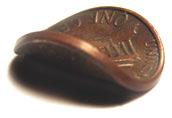
\includegraphics[width=1in]{bentcoin.jpg}
\label{fig:bentcoin}
\caption{Bent Coin}
\end{marginfigure}


Imagine we have a series of coins bent by various amounts (Figure~\ref{fig:bentcoin}).  If the coin is bent completely in half, then we could have the coin always flip heads (i.e. $\P{heads}=1$) or tails (i.e. $\P{tails}=1$) depending on how it is bent.  If you don't bend the coin at all then we'd have a fair coin ($\P{heads}=\P{tails}=0.5$).\marginnote{Why do we number them from zero here?  It's so that the number of the coin, say number 7, corresponds the probability that that coin flips heads, $\P{heads}=0.7$}
  So, let's say that we have a collection of bent coins which are bent by different amounts.  For convenience we will number them from 0 to 10.    The Table~\ref{tbl:bentcoin} summarizes the probability of each coin flipping heads.
\begin{table}
\begin{center}
\begin{tabular}{cc}
Coin Number & Probability for Flipping Heads ($\P{heads}$) \\ \hline\hline
0 & 0.0 \\
1 & 0.1 \\
2 & 0.2 \\
3 & 0.3 \\
4 & 0.4 \\
5 & 0.5 \\
6 & 0.6 \\
7 & 0.7 \\
8 & 0.8 \\
9 & 0.9 \\
10 & 1.0
\end{tabular}
\end{center}
\label{tbl:bentcoin}
\caption{Probabilities for flipping heads given a collection of bent coins}
\end{table}

Now I have the following scenario\cite{Lindley76}, with a few questions.
\begin{quote}
Imagine I have taken a random coin from my collection, flipped it and observed the following data:
\begin{center}
T T T H T H T T T T T H (i.e. 9 tails and 3 heads)
\end{center}
\be
\i From this data, which coin do I most likely have? 
\i  Can we be {\em significantly confident} that this particular coin will result in more tails than heads in the future?
\ee
\end{quote}

The way we've set up this problem is exactly like the model comparison example with the High and Low Deck (Section~\ref{sec:highlowdeck}), except in this case we have 11 models (one for each coin).  Applying the Bayes' Recipe we have
\be
\i Specify the prior probabilities for the models being considered.  Given no further information, we select a {\em uniform} distribution for the prior (i.e. all models are initially equally probable):
\beqn
P(M_{0})&=& 1/11 \\
P(M_{1})&=& 1/11 \\
&\vdots& \\
P(M_{10})&=& 1/11 \,.
\eeqn
where $M_{0}$ is the model defined by ``we're flipping coin 0,'' $M_{1}$ is the model defined by ``we're flipping coin 1,'' etc...
\i Write the top of Bayes' Rule for all models being considered:
\beqn
P(M_{0}|{\rm data}=9T,3H)&\sim&P({\rm data}=9T,3H|M_{0})P(M_{0})\\
P(M_{1}|{\rm data}=9T,3H)&\sim&P({\rm data}=9T,3H|M_{1})P(M_{1})\\
&\vdots& \\
P(M_{10}|{\rm data}=9T,3H)&\sim&P({\rm data}=9T,3H|M_{10})P(M_{10}) \,.
\eeqn
\i Put in the likelihood and prior values.  Here we are drawing from a {\em binomial} distribution for the likelihood:
\beqn
P(M_{0}|{\rm data}=9T,3H)&\sim&\nchoosek{12}{3}0.0^{3}\times (1-0.0)^{9}\times 1/11\\
P(M_{1}|{\rm data}=9T,3H)&\sim&\nchoosek{12}{3}0.1^{3}\times (1-0.1)^{9}\times 1/11\\
&\vdots& \\
P(M_{10}|{\rm data}=9T,3H)&\sim&\nchoosek{12}{3}1.0^{3}\times (1-1.0)^{9}\times 1/11 \,.
\eeqn
\i Add these values for all models: see Table~\ref{tbl:bentcoinprobs}.

\i Divide each of the values by this sum, $K$, to get the final probabilities: see Table~\ref{tbl:bentcoinprobs}.

\ee

\begin{table}
\begin{tabular}{ccc}
Model & $\sim P(M_i|{\rm data}=9T,3H)$ & $\sim P(M_i|{\rm data}=9T,3H)/K$ \\\hline\hline
$M_{0}$ & 0.000 & 0.000\\
$M_{1}$ & 0.00774 & 0.110\\
$M_{2}$ & 0.0214 & 0.306\\
$M_{3}$ & 0.0217 & 0.310\\
$M_{4}$ & 0.0128 & 0.184\\
$M_{5}$ & 0.00488 & 0.0696\\
$M_{6}$ & 0.00113 & 0.0161\\
$M_{7}$ & 0.000135 & 0.00192\\
$M_{8}$ & 0.00000524 & 0.0000748\\
$M_{9}$ & 0.0000000145 & 0.000000208\\
$M_{10}$ & 0.000 & 0.000\\
\cline{2-2}&$K$=0.0700 & 
\end{tabular}
\label{tbl:bentcoinprobs}
\caption{Probability for different bent-coin models, given the data={9 tails, 3 heads}.  The middle column is the non-normalized value from Bayes' Rule, needing to be divided by $K$ (the sum of the middle column) to get the final column which is the actual probability.}
\end{table}

When we are dealing with this many models, it is easier to plot the results, shown in Figure~\ref{fig:bentcoinprobs}.  We are now in a position to address the questions posed at the beginning of the section.

\begin{figure}
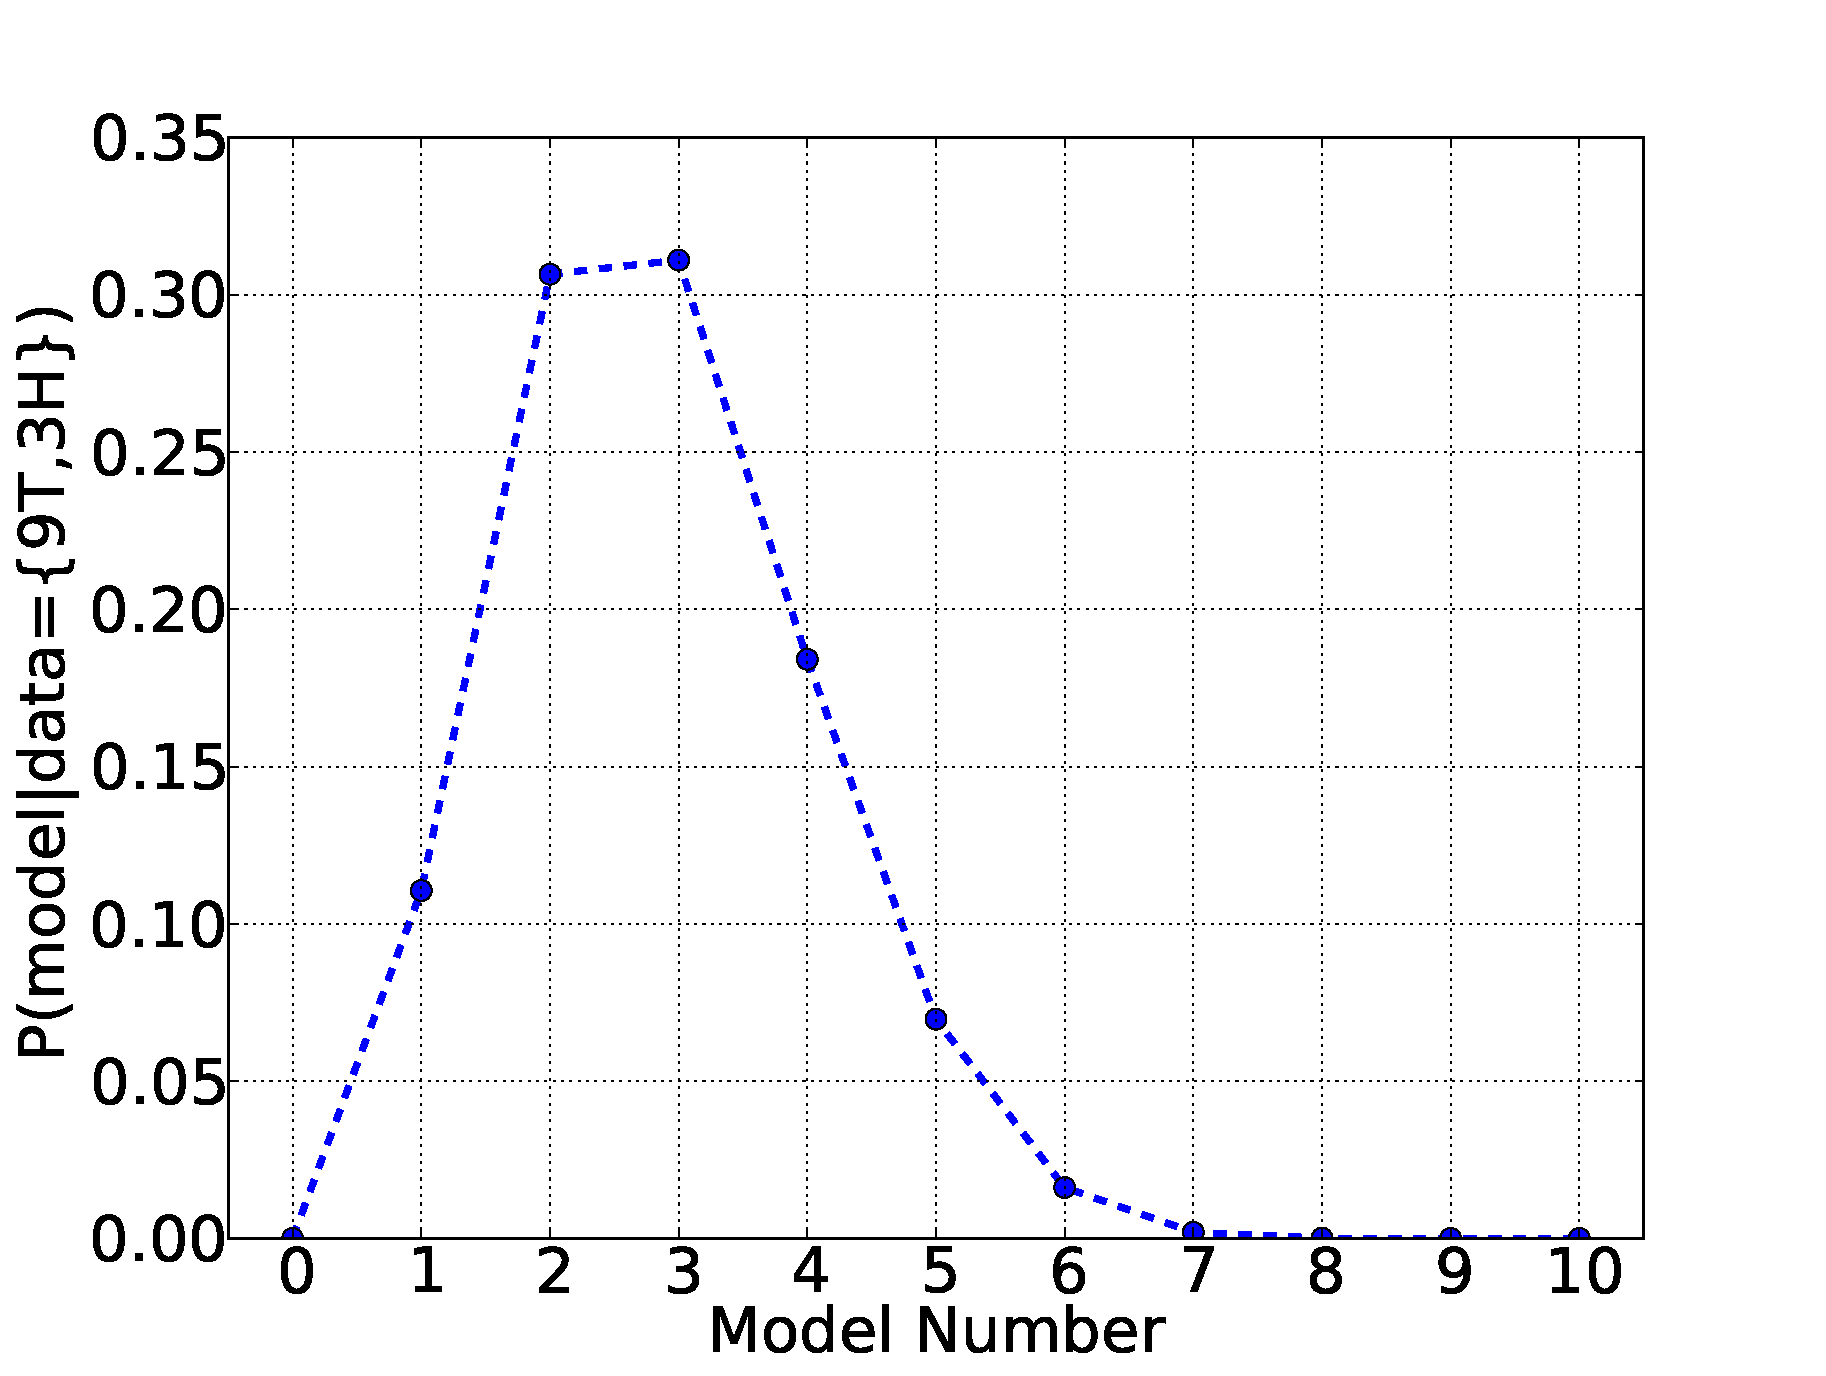
\includegraphics{bentcoinprobs1}
\label{fig:bentcoinprobs}
\caption{Probability for different bent-coin models, given the data={9 tails, 3 heads}.}
\end{figure}
\be
\i From this data, which coin do I most likely have? 

The maximum probability is for coin 3, but coin 2 is a close second.  Thus we can be reasonably confident that we have been flipping one of those two coins, but can't narrow our confidence any more than that.

\i  Can we be {\em significantly confident} that this particular coin will result in more tails than heads in the future?

This is another way of asking for the total probability for coins less than coin 5 (the fair coin), or
\beqn
\lefteqn{\P{coin 0 {\bf or} coin 1 {\bf or} coin 2 {\bf or} coin 3 {\bf or} coin 4}=}\\
&&0.000+0.110+0.306+0.310+0.184=0.912
\eeqn
which says that this coin is ``likely'' to ``very likely'' (Table~\ref{table1} on page~\pageref{table1}) to have a probability of yielding heads less than a fair coin, and thus yield more tails in the future.
\ee



\section{Priors versus Data}

It is instructive to pause and look at this example one flip at a time, to see how the probability and thus our state of knowledge adjusts as we collect more data.  In Figure~\ref{fig:bentcoinprobs2} we see the result of our procedure when there is no data (i.e. our initial, prior probabilities) and when we've flipped once and then again, both times tails.  The curve for ``no data'' is the same as the prior probability, and in this case all models are equally likely.  When the first tails is observed, the model which states that heads are {\em certain} (i.e. coin 10) goes to zero probability because coin 10 \emph{cannot} flip tails.\footnote{Notice that the only models with probability equal to zero are ones that are \emph{logically impossible}.  It's not the colloquial usage of impossible, as in ``it is impossible for the Red Sox to win this year,'' but in the strict usage, as in ``it is impossible to flip both heads and tails at the same time.''  The reason this is the case is that a statement with zero probability cannot be made possible with \emph{any about of data} - it is an utterly \emph{dogmatic} statement.  Thus, we reserve it only for things that are \emph{logically impossible}.
}.  At this point we {\em know} that it is {\em impossible} for us to be flipping coin 10.  We see also that the high-numbered coins (i.e. the ones with high probability of flipping heads) have greatly reduced probability while we've seen only tails.

As more tails are observed, the probability for the lower models is increased.  As we flip more tails we become more confident in the lower-number models.  Because at this point we haven't flipped any heads, the model 0 still has non-zero probability - it is still possible that we are holding a coin that cannot flip heads.

\begin{figure*}
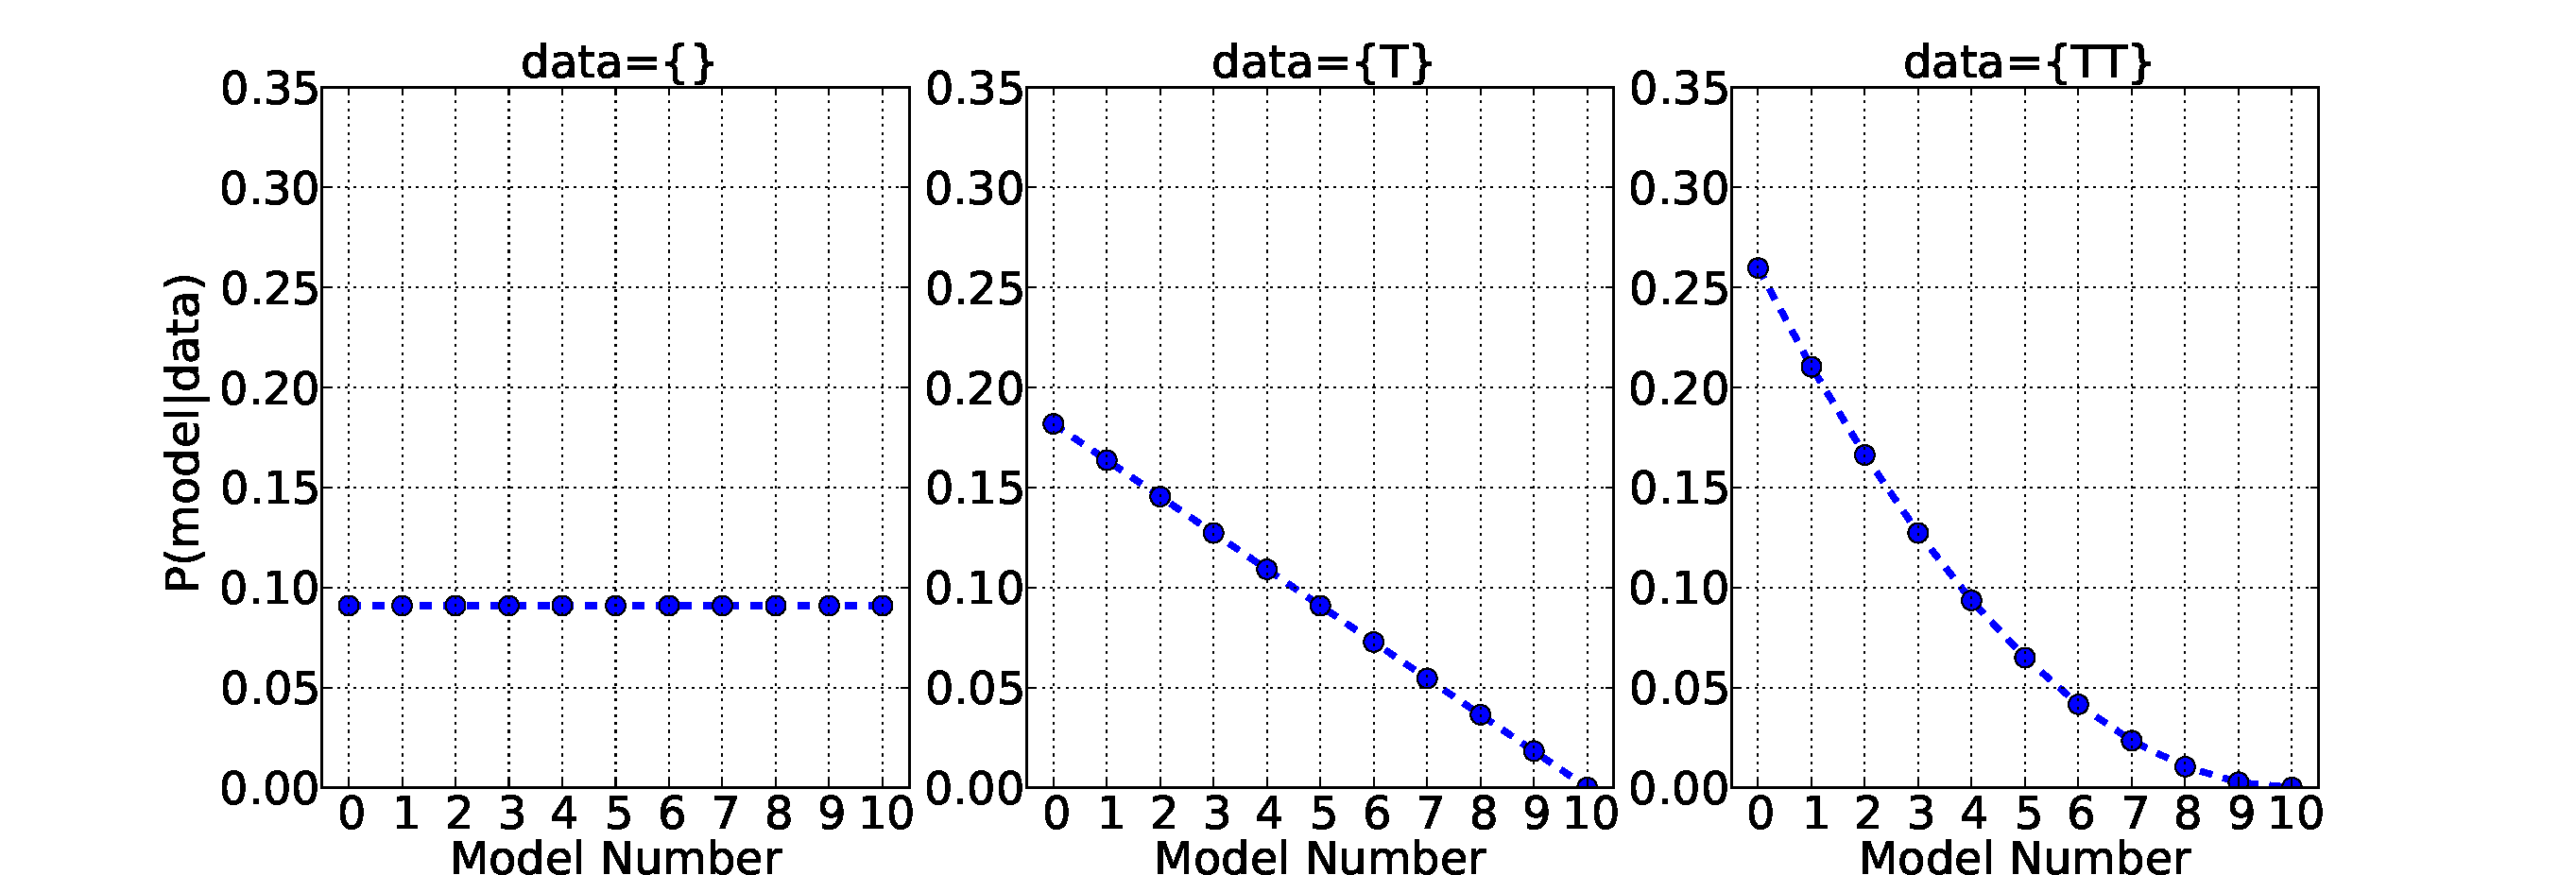
\includegraphics{bentcoinprobs2}
\label{fig:bentcoinprobs2}
\caption{Probability for different bent-coin models, given no data (left), the first tails (middle), and the second tails (right).  The curve for no data is the same as the prior probability, and in this case all models are equally likely.  When the first tails is observed, the model which states that heads are {\em certain} (coin 10) goes to zero probability.  As more tails are observed, the probability for the lower models is increased.}
\end{figure*}

When we continue with the next few flips (Figure~\ref{fig:bentcoinprobs3}) we encounter our first heads on the fourth flip.  At this point the model which states that heads are {\em impossible} (i.e coin 0) goes to \emph{zero} probability.  Finally, across our entire data set (Figure~\ref{fig:bentcoinprobs5}) we see that the curve gets narrower, where more of the probability falls on only a few of the models and the other models become less and less likely.  With only 12 data points, there is still a lot of uncertainty in which model - several models have reasonably high probability values.  We still can rule out a few models confidently (like coins 0, 6, 7, 8, 9, and 10).  We are most confident in coins 2 and 3, with the most probability. 

\vspace{1in}
\begin{figure*}
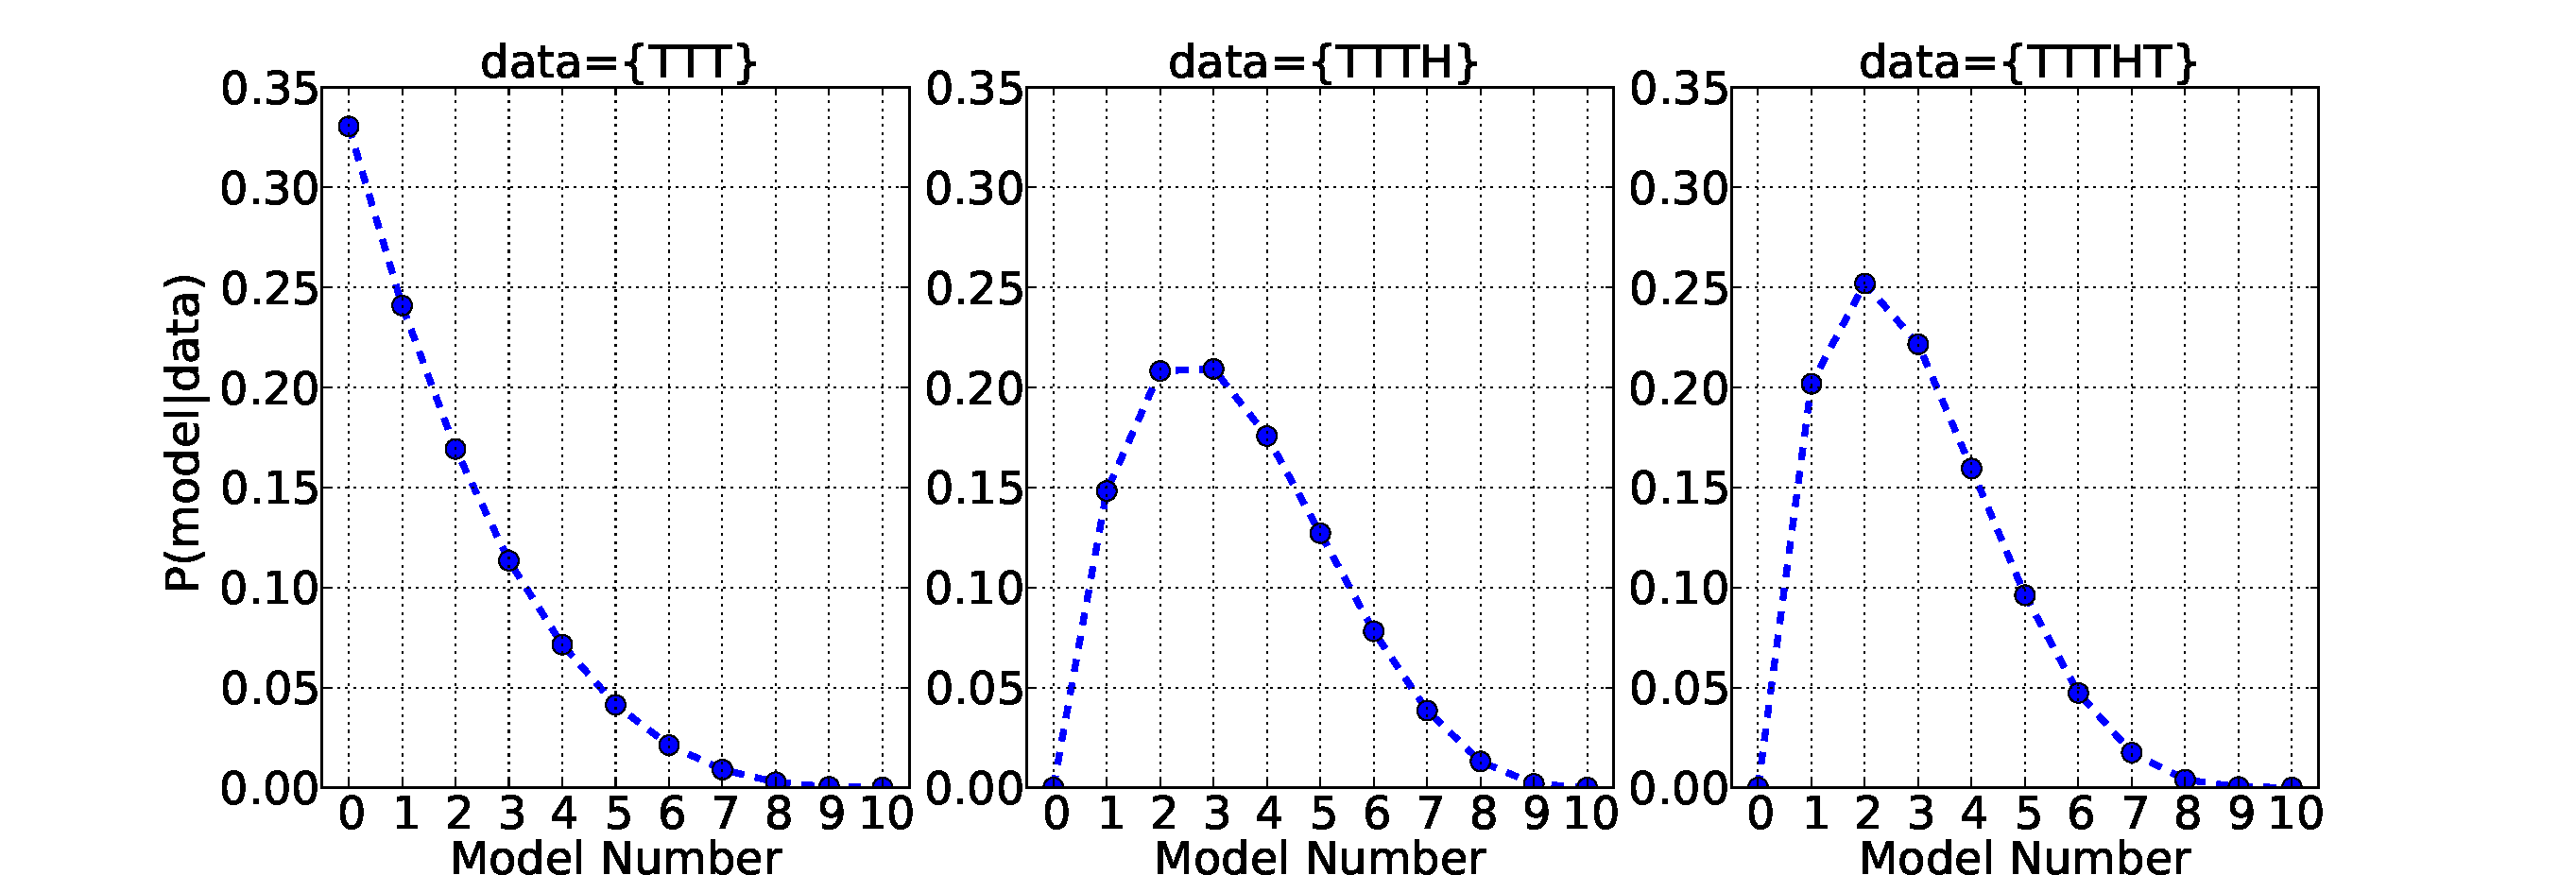
\includegraphics{bentcoinprobs3}
\label{fig:bentcoinprobs3}
\caption{Probability for different bent-coin models, given three tails (left), the first heads (middle), and another tails (right).  When the first heads is observed, the model which states that heads are {\em impossible} (coin 0) goes to zero probability.}
\end{figure*}





\begin{figure*}
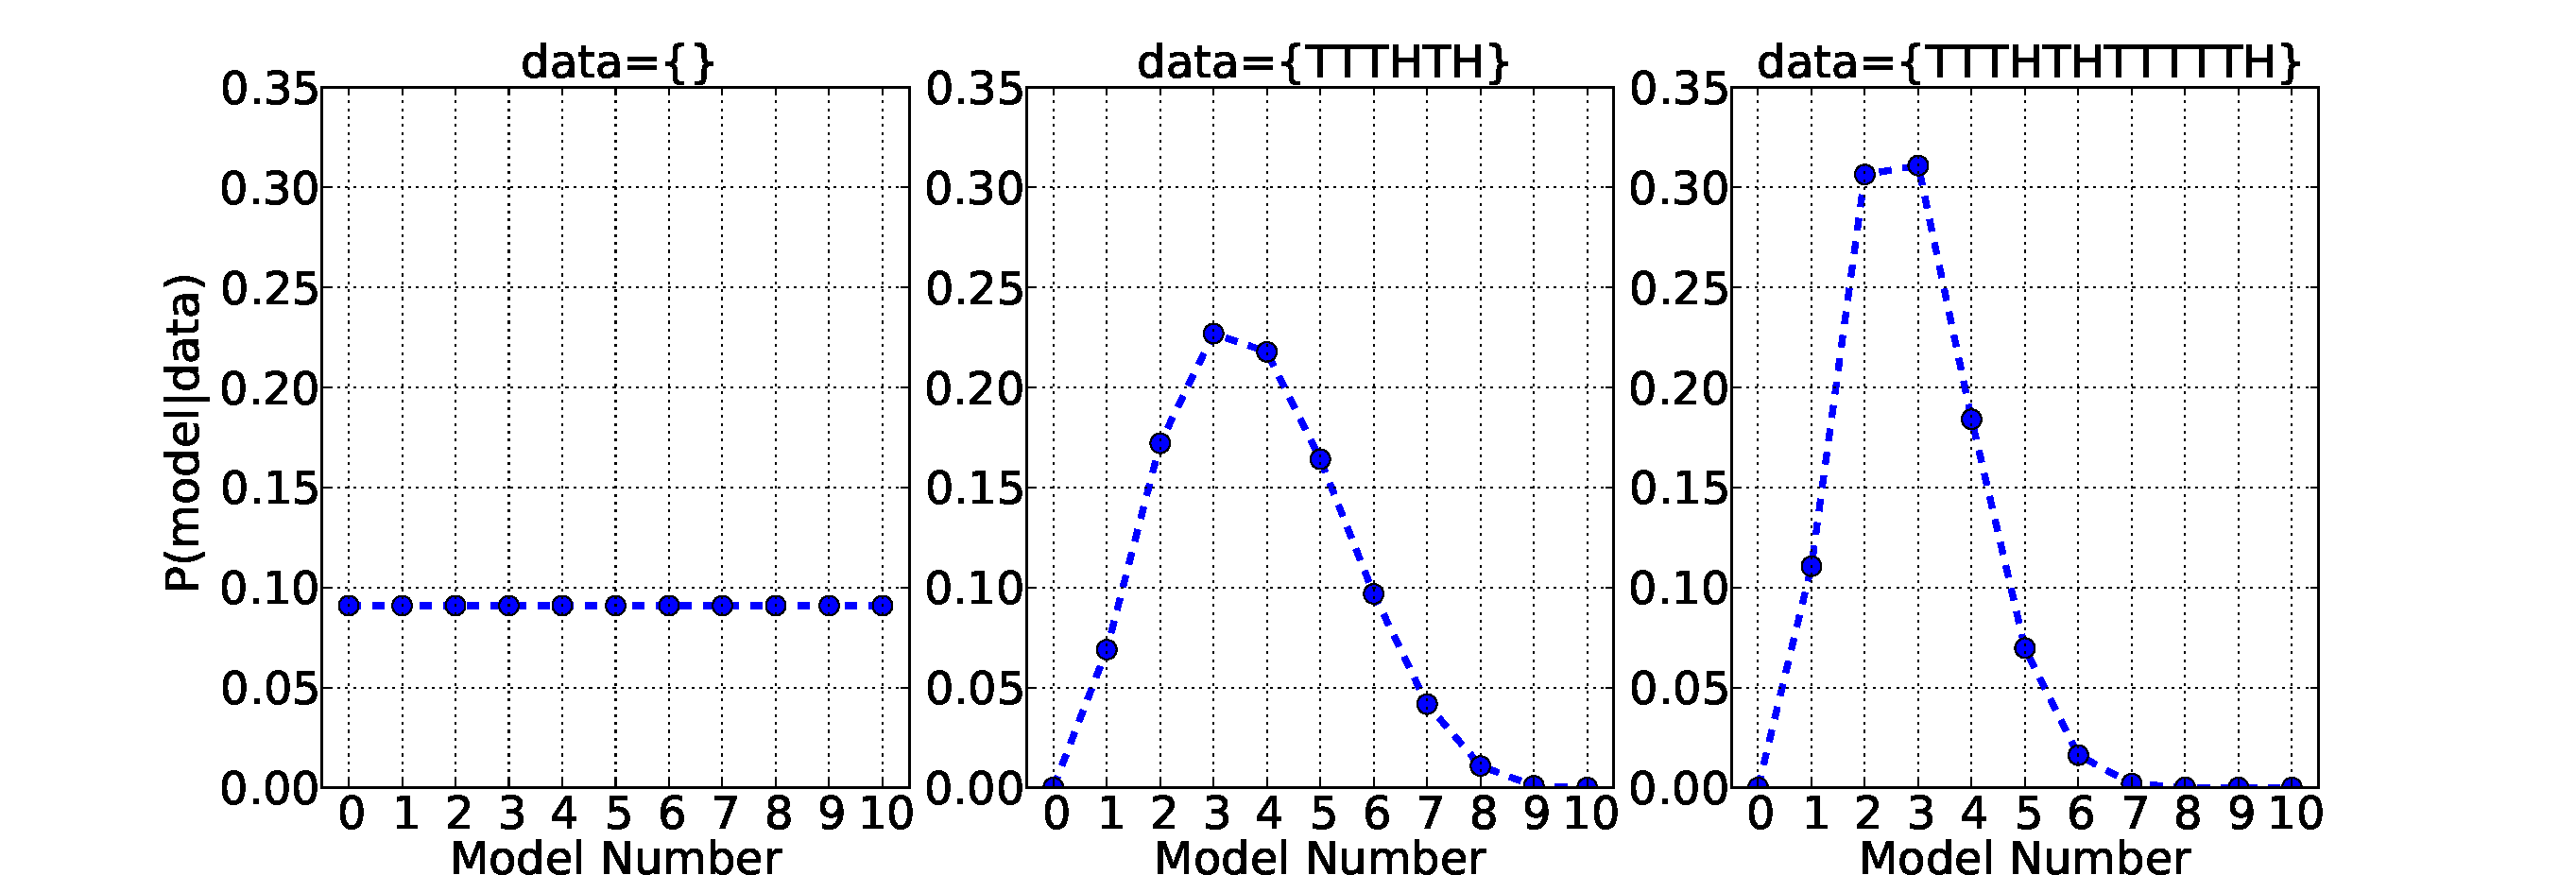
\includegraphics{bentcoinprobs5}
\label{fig:bentcoinprobs5}
\caption{Probability for different bent-coin models, given no data (left), the first half of the data set (middle), and the entire data set of 9 tails and 3 heads (right).}
\end{figure*}



\section{Moving Toward the Continuous}\label{sec:continuous}

There is a practical problem that we face at this point, when we consider a generic bent coin.  Perhaps it doesn't fit in one of the 11 models considered, falling somewhere in between, for example with $\P{heads}=0.132464$. Ones' first thought might be to include one thousand coins or one million coins instead of the 11 we've considered so far, so we could have coin 132464, coin 132465, coin 132466, etc...  Although this can be done, we run into two problems
\be
\i Because we are dealing with so many models, the probability associated with any \emph{single} model gets very small - and gets smaller with the more models you consider
\i We can't practically distinguish between models such as $\P{heads}=0.132464$ and $\P{heads}=0.13246{\bf 5}$ (the last digit is different here)
\ee

In order to solve both of these problems mathematically, we introduce the concept of a {\em continuous distribution}.  We start by labeling the model with a {\em continuous} number rather than an integer.  In our present case it makes sense to label the model with the probability that the coin flips heads.  We'll call this label $\theta$, and it will have a value between 0 (heads are impossible) and 1 (heads are certain) and can take on {\em any value} in between.  Because we now have an infinite number of labels, we have two consequences:
\be
\i We can't simply add up all the probabilities to get our value of $K$ to make everything add up to 1.  Instead, we look at {\em areas under the curve} and make sure the entire area equals 1.
\i Because, with distributions, \emph{areas under the curve} (and not the values of the distribution itself) are the probabilities, we can only speak about {\em ranges} of values.  For example, we can speak meaningfully about the probability of $\theta$ between 0.3 and 0.4 (i.e. $P(0.3<\theta<0.4)$).  When we write down something like $P(\theta)=1$ we're not talking about a probability of a single label but rather the magnitude of the distribution at that label, $\theta$.
\ee

We revisit Bayes' Recipe again, using the distributions.  This time we also will look at pictures of the distributions as we progress.

\be
\i Specify the prior probabilities for the models being considered:
\beqn
P(\theta) = 1 \,.
\eeqn
\begin{marginfigure}
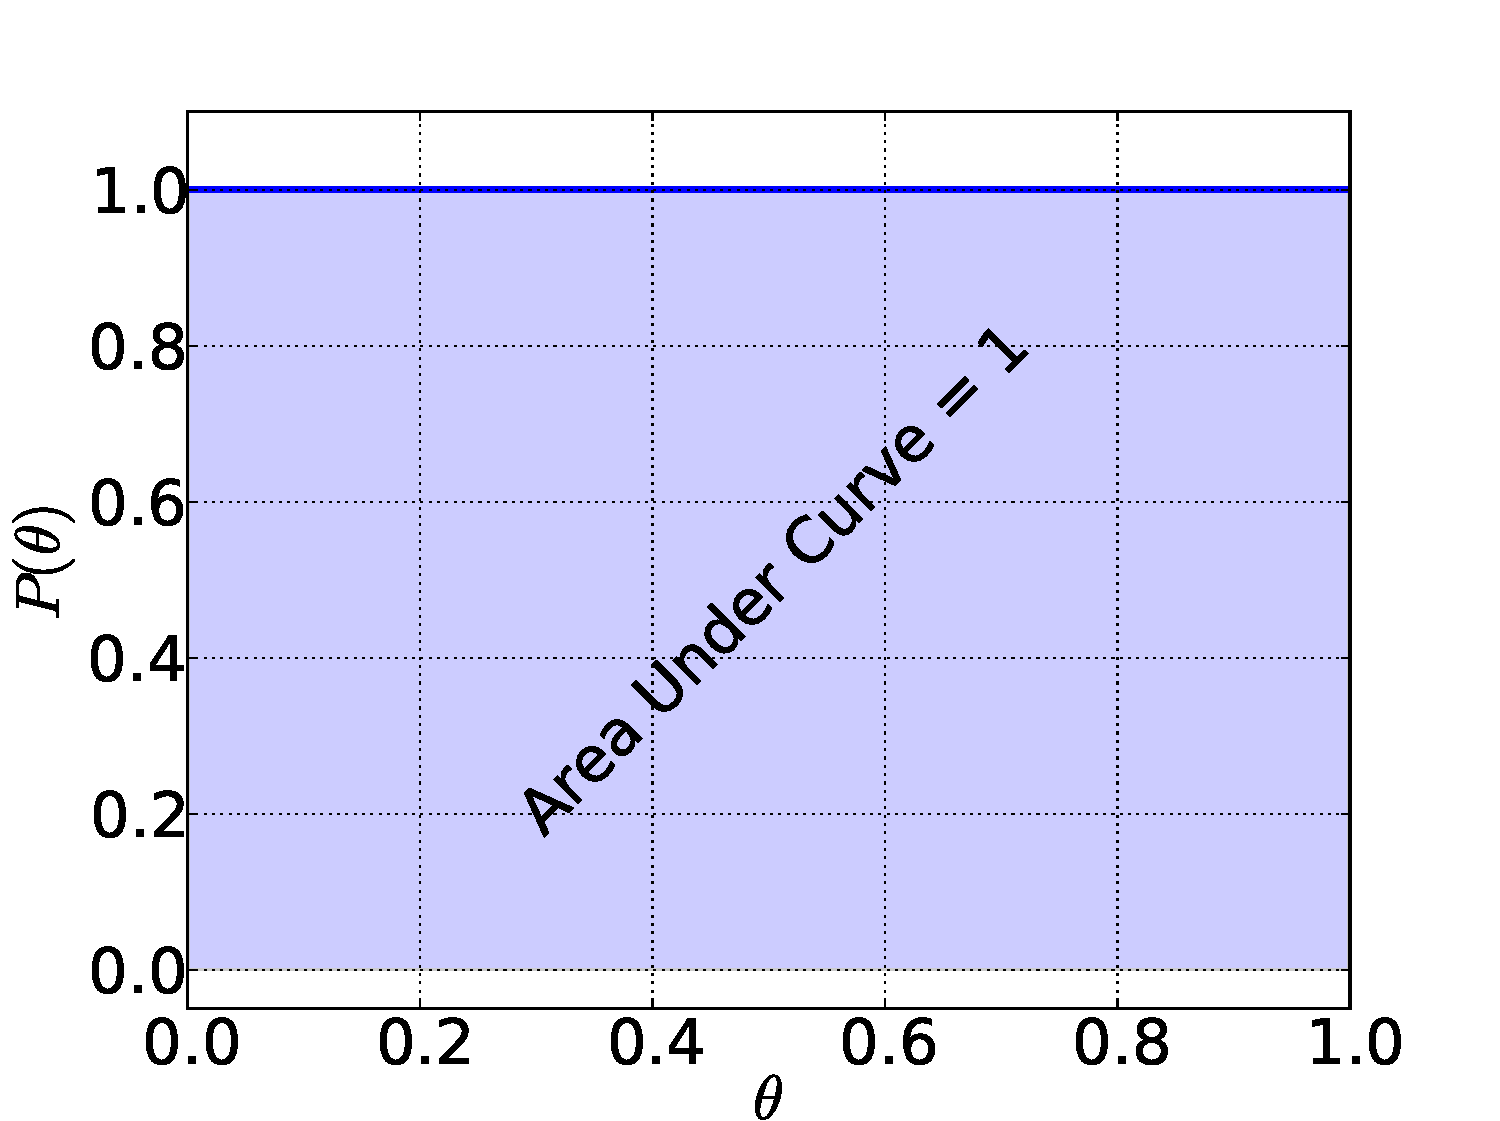
\includegraphics{bentcoindist1}
\end{marginfigure}

\i Write the top of Bayes' Rule for all models being considered:

We can write one equation for all of the models labeled by $\theta$ at once as

\beqn
P(\theta|{\rm data}=9T,3H)&\sim&P({\rm data}=9T,3H|\theta)P(\theta) \,.
\eeqn

\i Put in the likelihood and prior values.

We use the binomial model, one equation for all models, remembering that for a model labeled by $\theta$ the probability for that coin flipping heads is $\P{heads}=\theta$.  Thus we get the likelihood and prior values as
\beqn
P(\theta|{\rm data})&\sim&P({\rm data}|\theta) \cdot P(\theta)\\
P(\theta|{\rm data}9T,3H)&\sim&\nchoosek{12}{3}\theta^{3}\times (1-\theta)^{9} \cdot 1
\eeqn
\begin{marginfigure}
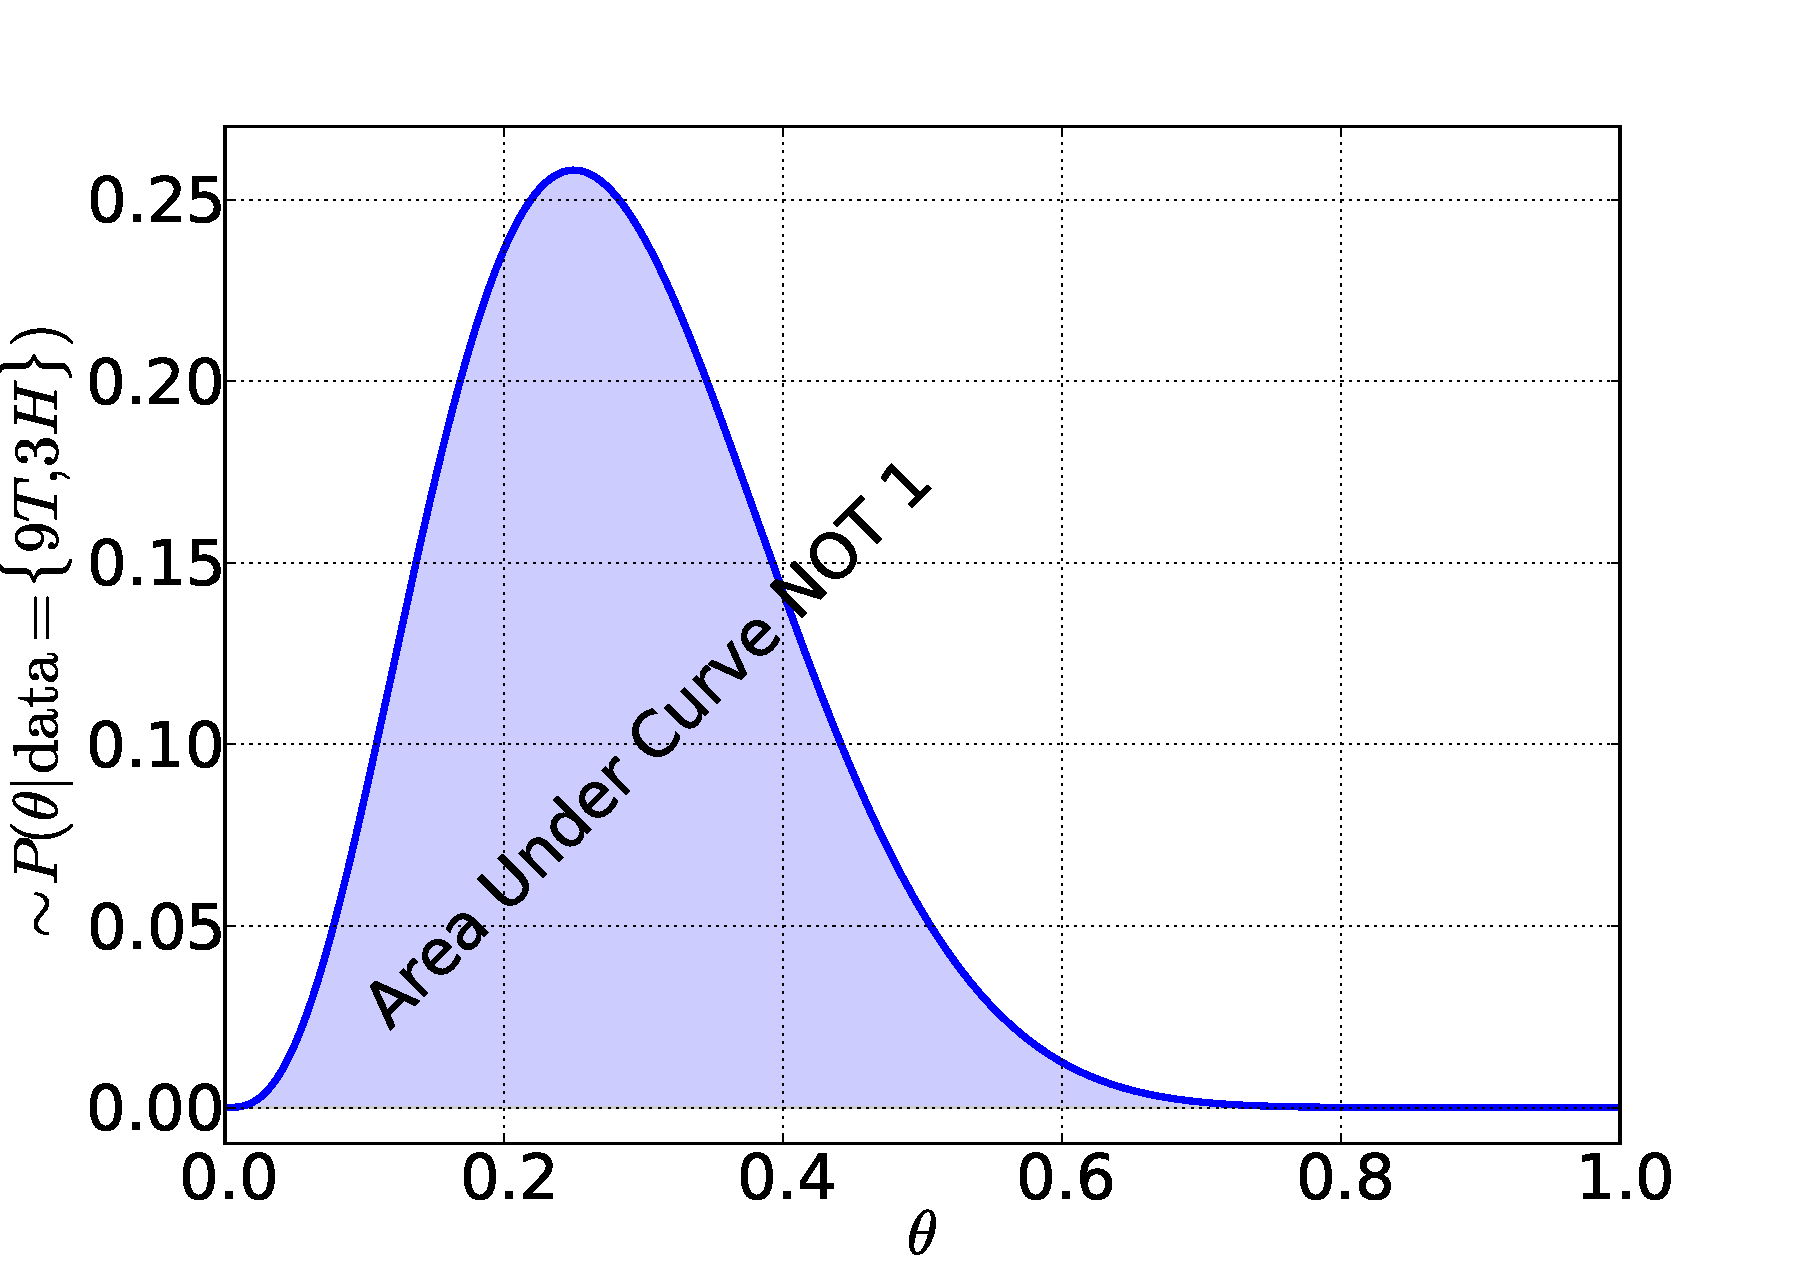
\includegraphics{bentcoindist2}
\end{marginfigure}

\i Find the area under this curve, and call it $K$.
\i Divide each of the values of the curve by this are, $K$, to get the final probabilities where the area under the curve is 1.
\begin{marginfigure}
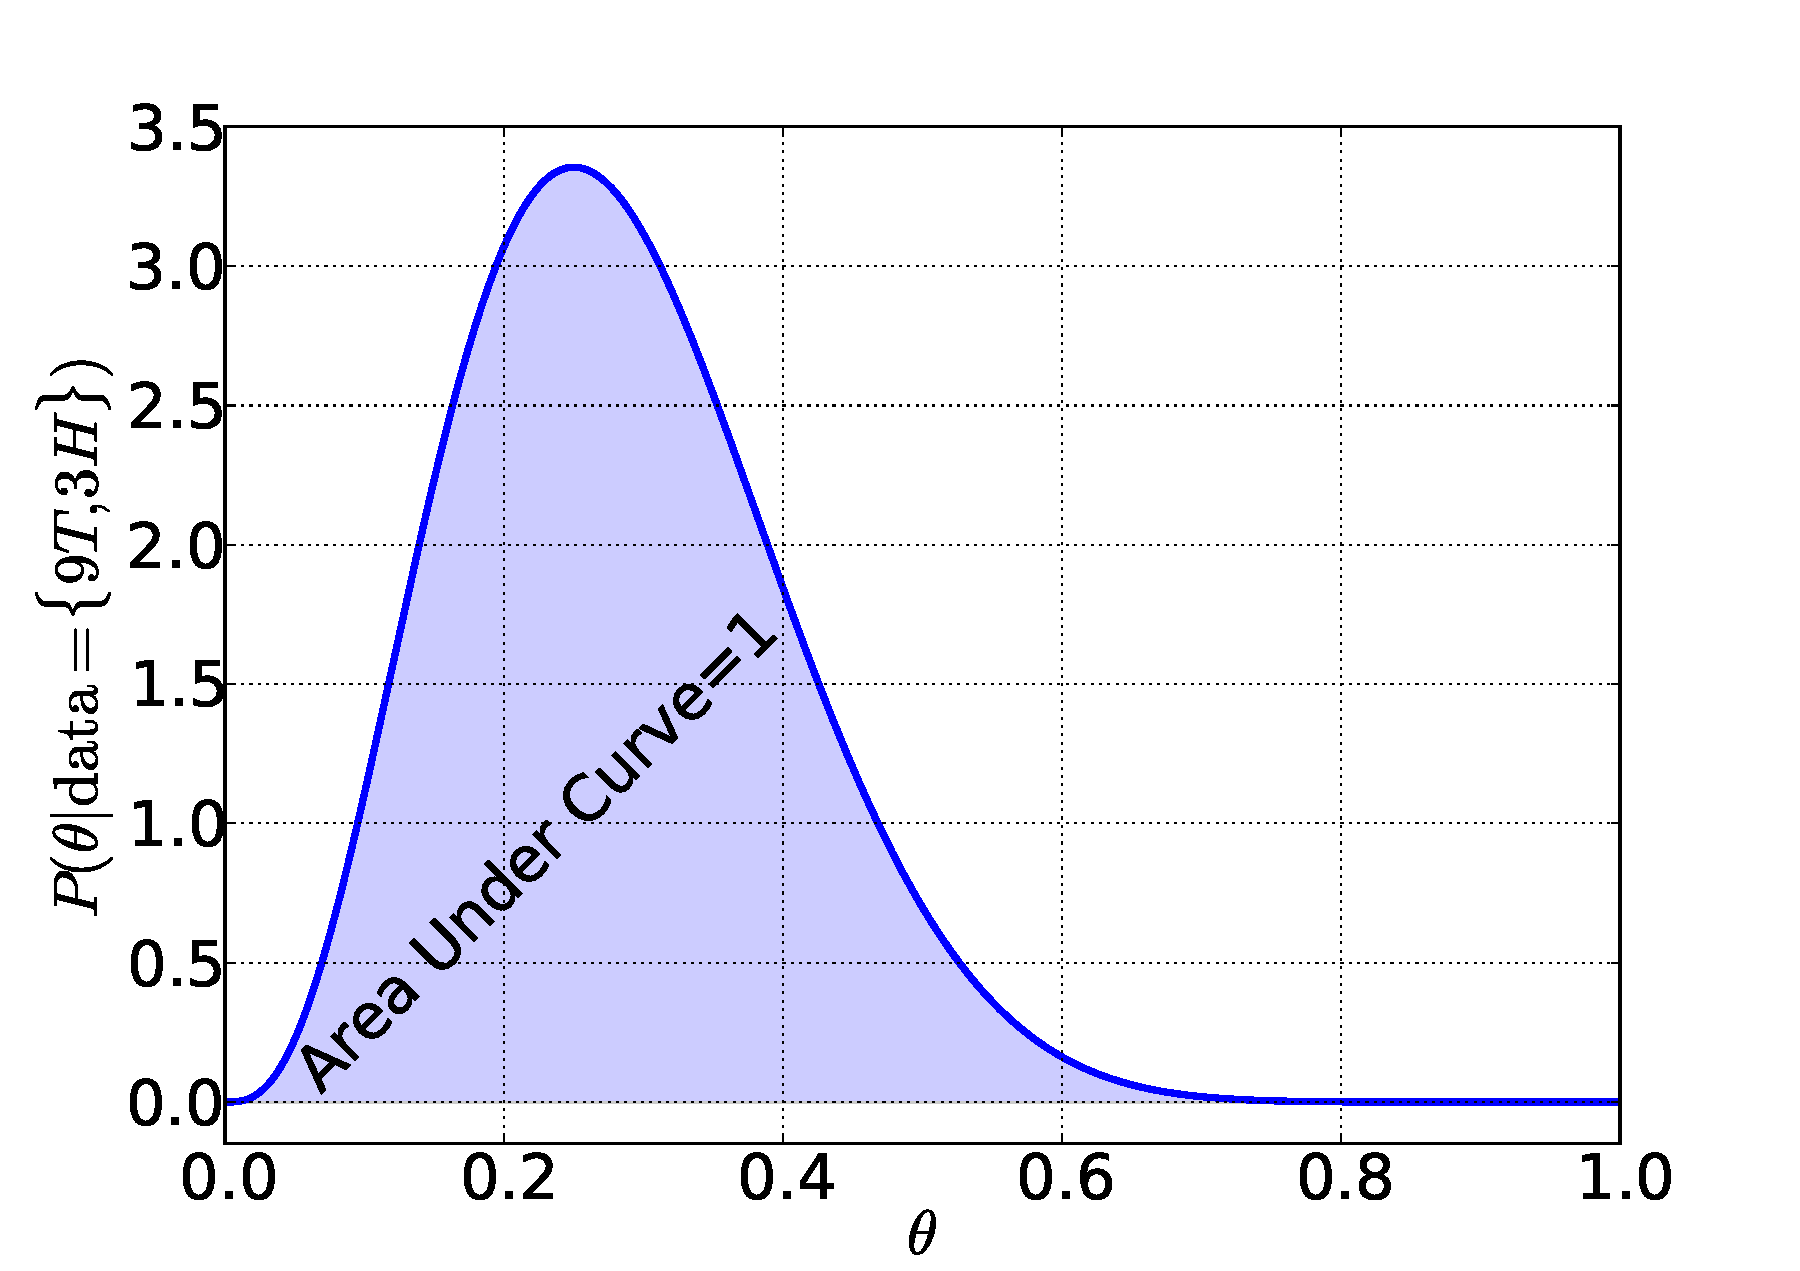
\includegraphics{bentcoindist3}
\end{marginfigure}
\ee

Usually these steps are done for you, for a specific data set, and you are given the final posterior distribution to use in answering any questions.  However, for any particular case it is important to know what assumptions have been made in the choice of models and model parameters.  

\section{MAP and Areas}

Now we revisit the questions posed in Section~\ref{sec:intro_bent_coin} on page~\pageref{sec:intro_bent_coin} about the bent coin, this time using the distribution found above, reproduced here in Figure~\ref{fig:coin_12_3_posterior}.

\begin{quote}
Imagine I have taken a random coin from my collection, flipped it and got the following data:
\begin{center}
T T T H T H T T T T T H (i.e. 9 tails and 3 heads)
\end{center}
\be
\i From this data, which ``coin'' do I most likely have? (or in this interpretation, what is my best estimate for the probability of this coin flipping heads, denoted by $\theta$)
\i Can we be {\em significantly confident} that this particular coin will result in more tails than heads in the future?
\ee
\end{quote}

\begin{figure}
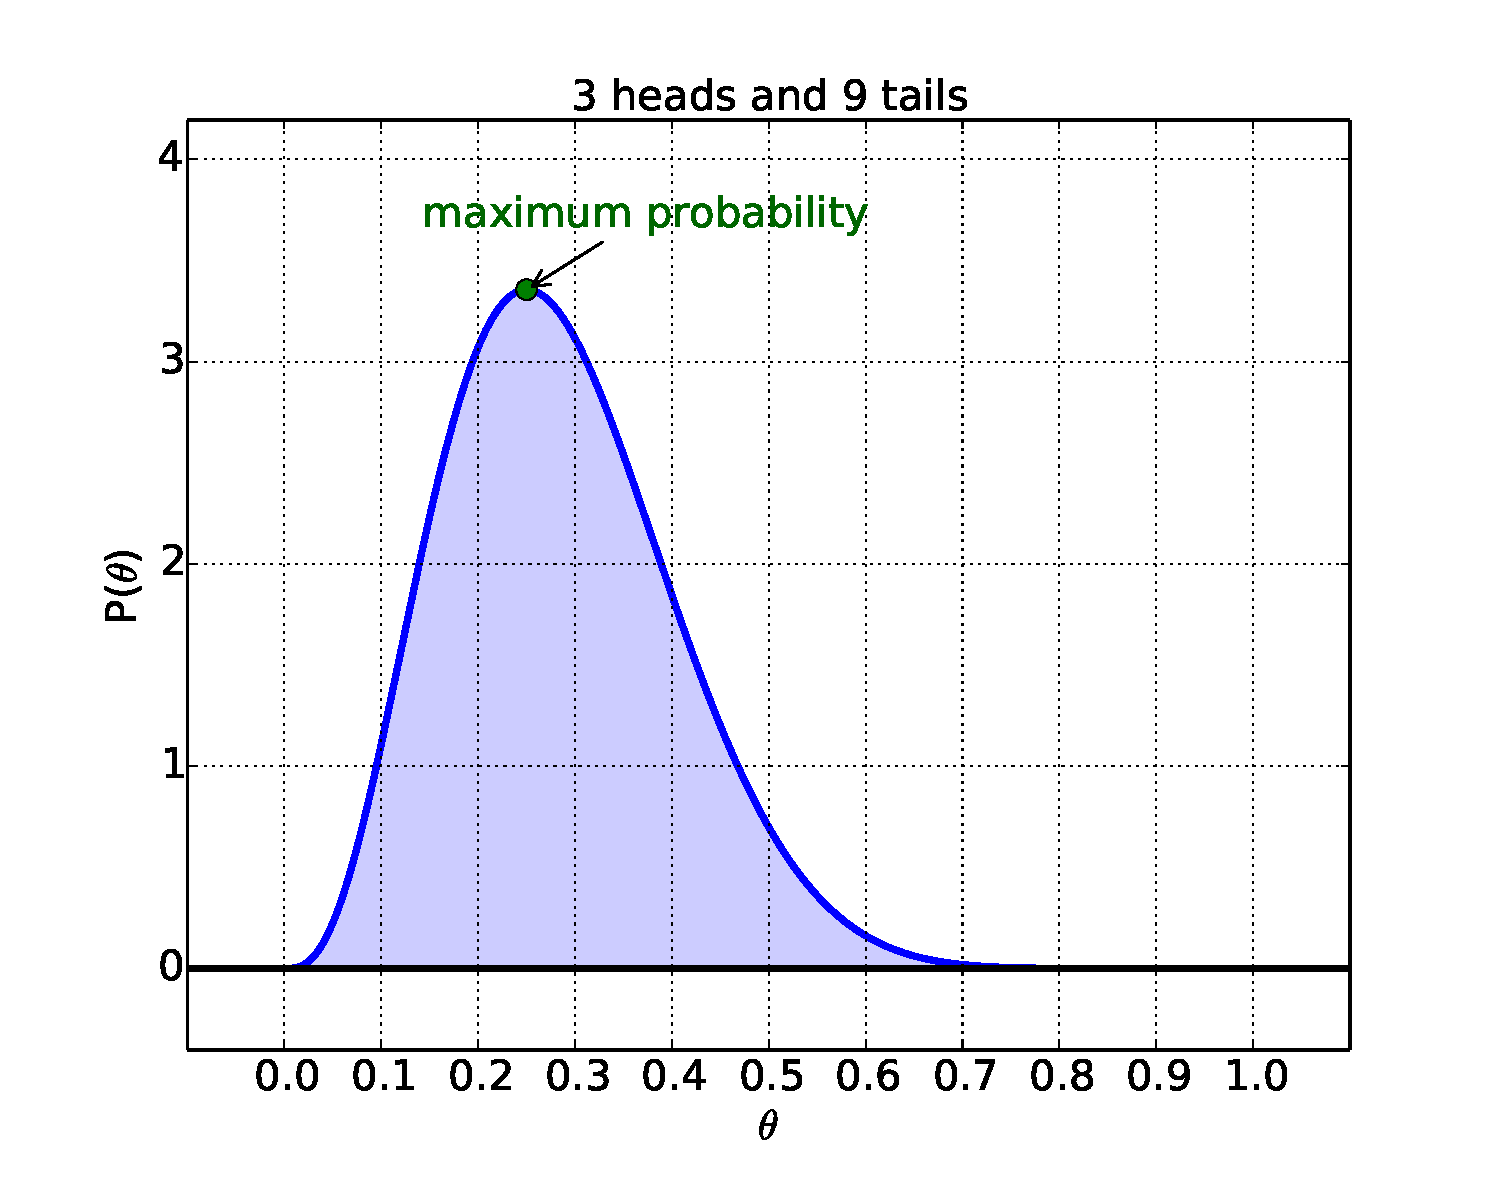
\includegraphics{beta_dist}
\caption{Posterior probability distribution for the $\theta$ values of the bent coin - the probability that the coin will land heads.  The distribution is shown for data 3 heads and 9 tails, with a maximum at $\theta=0.25$.}
\label{fig:coin_12_3_posterior}
\end{figure}

One answer to the first question can be accomplished by looking at the {\em maximum} of the posterior distribution, shown in Figure~\ref{fig:coin_12_3_posterior}.\footnote{The maximum of the posterior distribution, which represents the most likely value of a quantity, is often referred to as the {\em MAP estimate}.  It is also commonly referred to as the {\em mode} of the distribution.}  By eye, it seems to have a maximum at $\theta=0.25$.  In fact one can demonstrate that this distribution has a maximum at 
\beqn
\theta_{\rm max}=\frac{\mbox{number of successes}}{\mbox{total number of attempts}} \,,
\eeqn
where in our example, a success is head, and an attempt is a flip.\footnote{This distribution, given how common it is, is given the name {\em Beta distribution}.  There are a handful of common distributions that are given names for convenience.  We've already seen the {\em uniform distribution}, and there will be others.}  We take up this question of the best estimate of $\theta$, given the posterior probability for $\theta$, in more detail in Section~\ref{sec:bestest}.

The answer to the second question can be done by looking at the area under the curve from  $\theta=0$ , the ``all heads'' coin, to $\theta=0.5$, the ``fair'' coin, as shown in Figure~\ref{fig:coin_12_3_posterior_significance}.  This area represents the probability, given the data, that the coin is skewed towards heads or, in other words, how confident are we that this is an unfair coin.  Given the value of $P(\theta<0.5) = 0.954$ we can say that this is ``very likely'' an unfair coin (see Table~\ref{table1} on page~\pageref{table1}). 


\begin{figure}
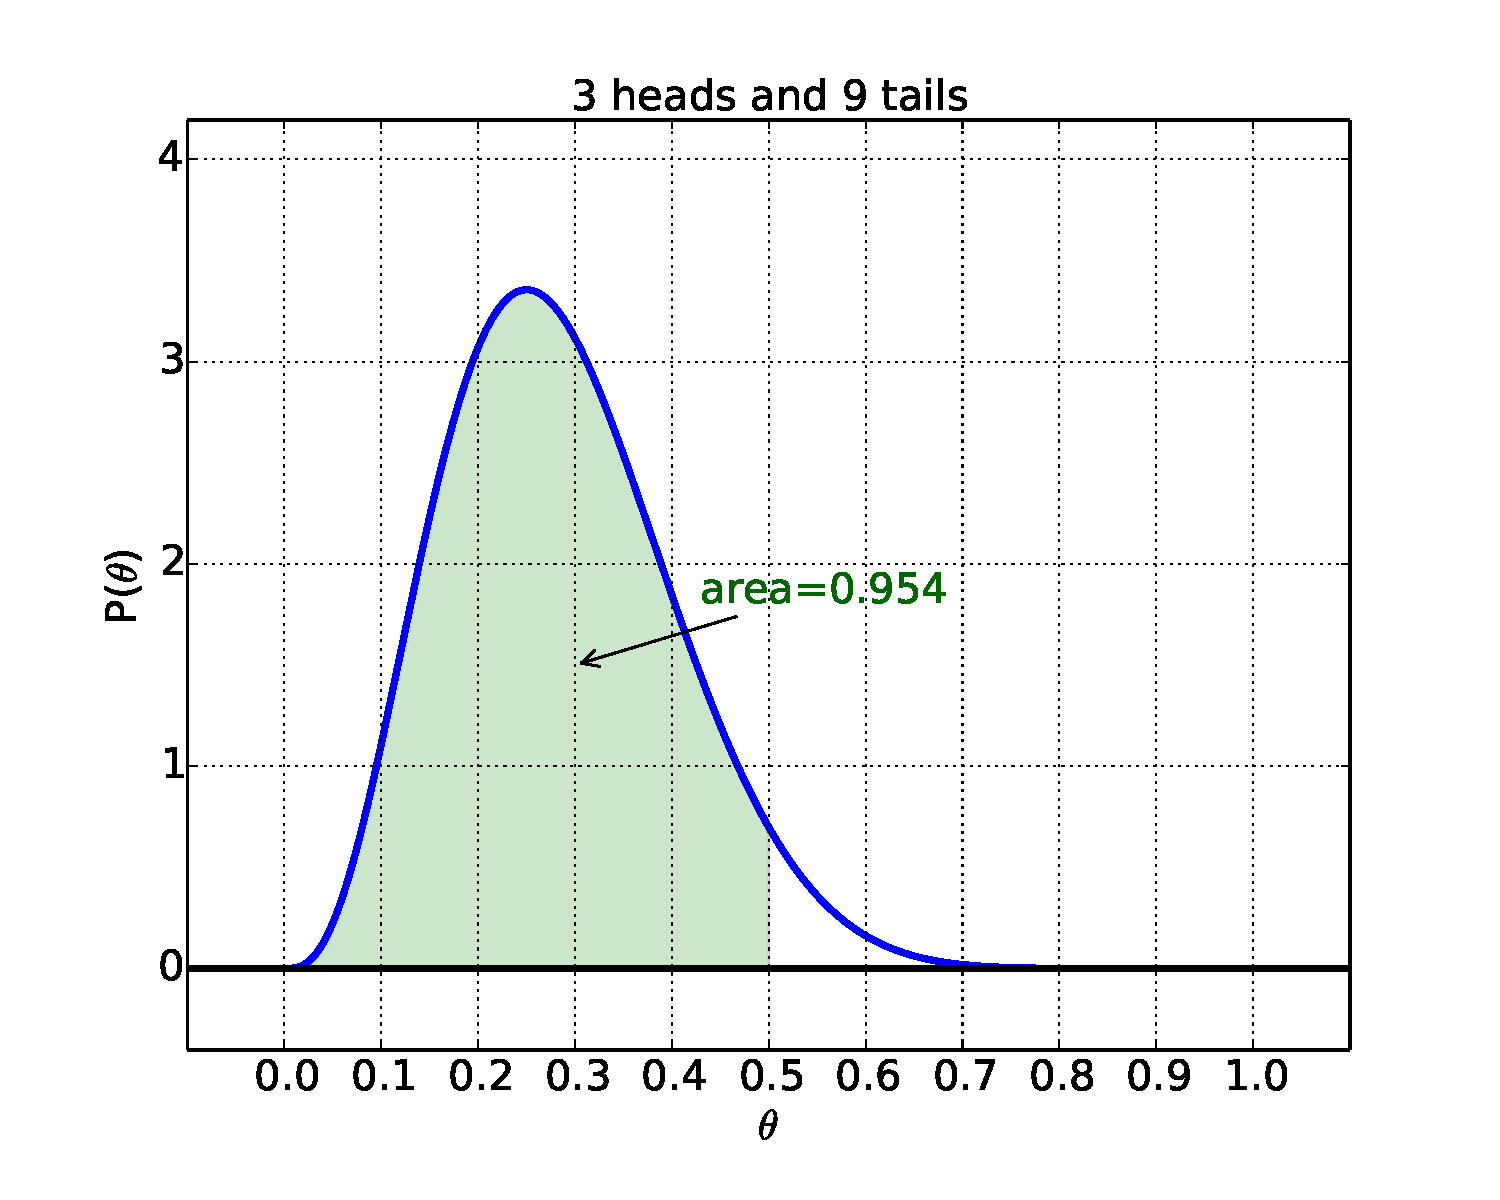
\includegraphics{beta_dist2}
\caption{Posterior probability distribution for the $\theta$ values of the bent coin - the probability that the coin will land heads.  The distribution is shown for data 3 heads and 9 tails.  The area under the curve from  $\theta=0$ (the ``all heads'' coin) to $\theta=0.5$ (the ``fair'' coin) is 0.954.}
\label{fig:coin_12_3_posterior_significance}
\end{figure}

\section{Quartiles}

Given that we are dealing most often with continuous distributions, and thus need to look at areas under the curve from one point to another, it is useful to make a table for a distribution of these areas.  Typically we look at the values of the parameter at which we have a given area under the curve from the minimum possible value of the parameter up to to that value.  For example, we might be interested in the value of $\theta$ (i.e. how skewed the coin is) such that we have an area of 50\% from 0 up to $\theta$, shown in Figure~\ref{fig:coin_12_3_posterior_median}. This point (called the {\em median}) represents the point where we would be just as confident (given our data) that the coin is {\em more} skewed than this as {\em less} skewed.  

\begin{figure}
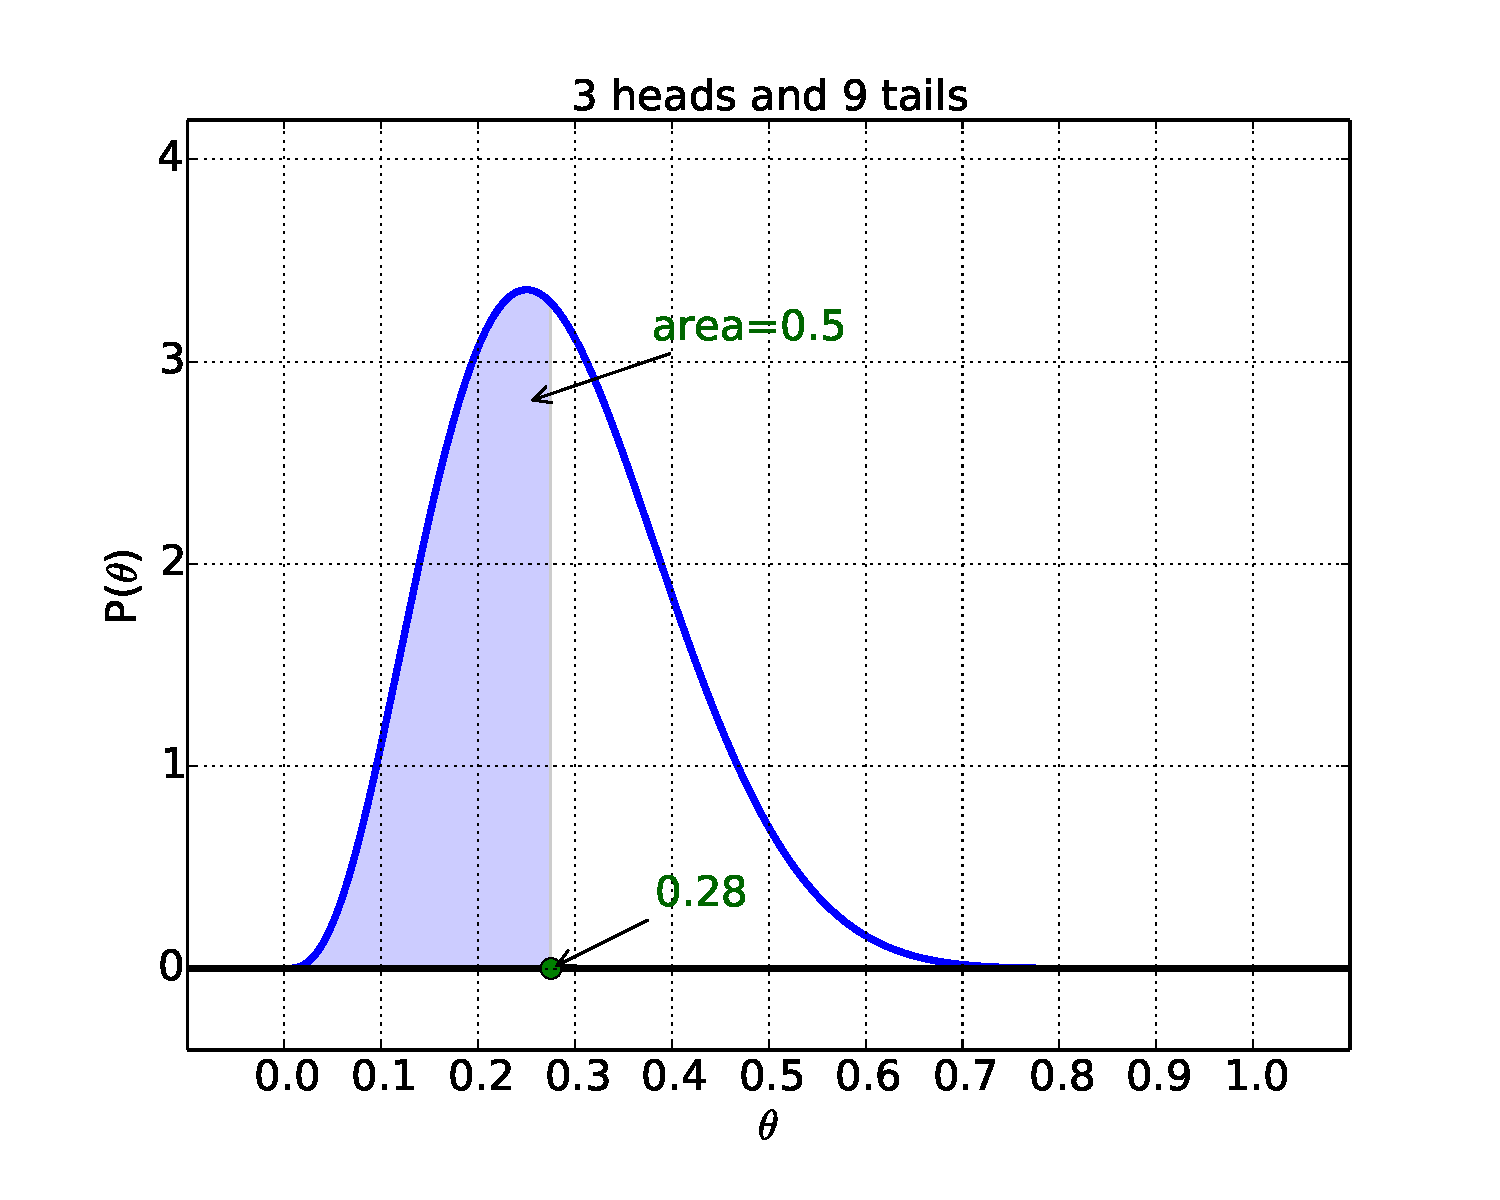
\includegraphics{beta_dist3}
\caption{Posterior probability distribution for the $\theta$ values of the bent coin - the probability that the coin will land heads.  The distribution is shown for data 3 heads and 9 tails.  The area under the curve from  $\theta=0$ (the ``all heads'' coin) to $\theta=0.28$ is 0.5 - half the area.  This represents the {\em median} of the distribution.}
\label{fig:coin_12_3_posterior_median}
\end{figure}

A table of these values for a distribution can be very useful.  For example, consider the table and plot shown in Figure~\ref{fig:coin_12_3_posterior_quartiles}.  Shown are the various points where the area under the curve up to those points is specified.  For example, the area under the curve from $\theta=0$ up to $\theta=0.11$ is 5\%.  This means, given the data of 3 heads and 9 tails, there is a probability $P=5\%$ of the coin having less than $\theta=0.11$, or an extreme skew towards tails.  \highlight{Quartiles}{The term {\em quartiles} refers to the values of the parameter which result in an area of 25\%, 50\%, or 75\%, or one, two, or three quarters of the area.}{The term {\em quartiles} refers to the values of the parameter which result in an area of 25\%, 50\%, or 75\%, or one, two, or three quarters of the area.}  When we wish to refer to a non-quarter percentage, then we'll call it a {\em percentile.}  \highlight{Percentiles}{The term {\em percentile} refers to the value of the parameter which result in a particulare area under the curve.}{The term {\em percentile} refers to the value of the parameter which result in a particulare area under the curve.}    For example, we can say from Figure~\ref{fig:coin_12_3_posterior_quartiles} that the 99\% percentile is 0.59.  Thus, it is extremely unlikely to have the coin skewed towards heads more than $\theta=0.59$ given the observation that we flipped 3 heads and 9 tails with this coin.


\begin{figure*}
\begin{tabular}{cp{1in}}
\raisebox{-2in}{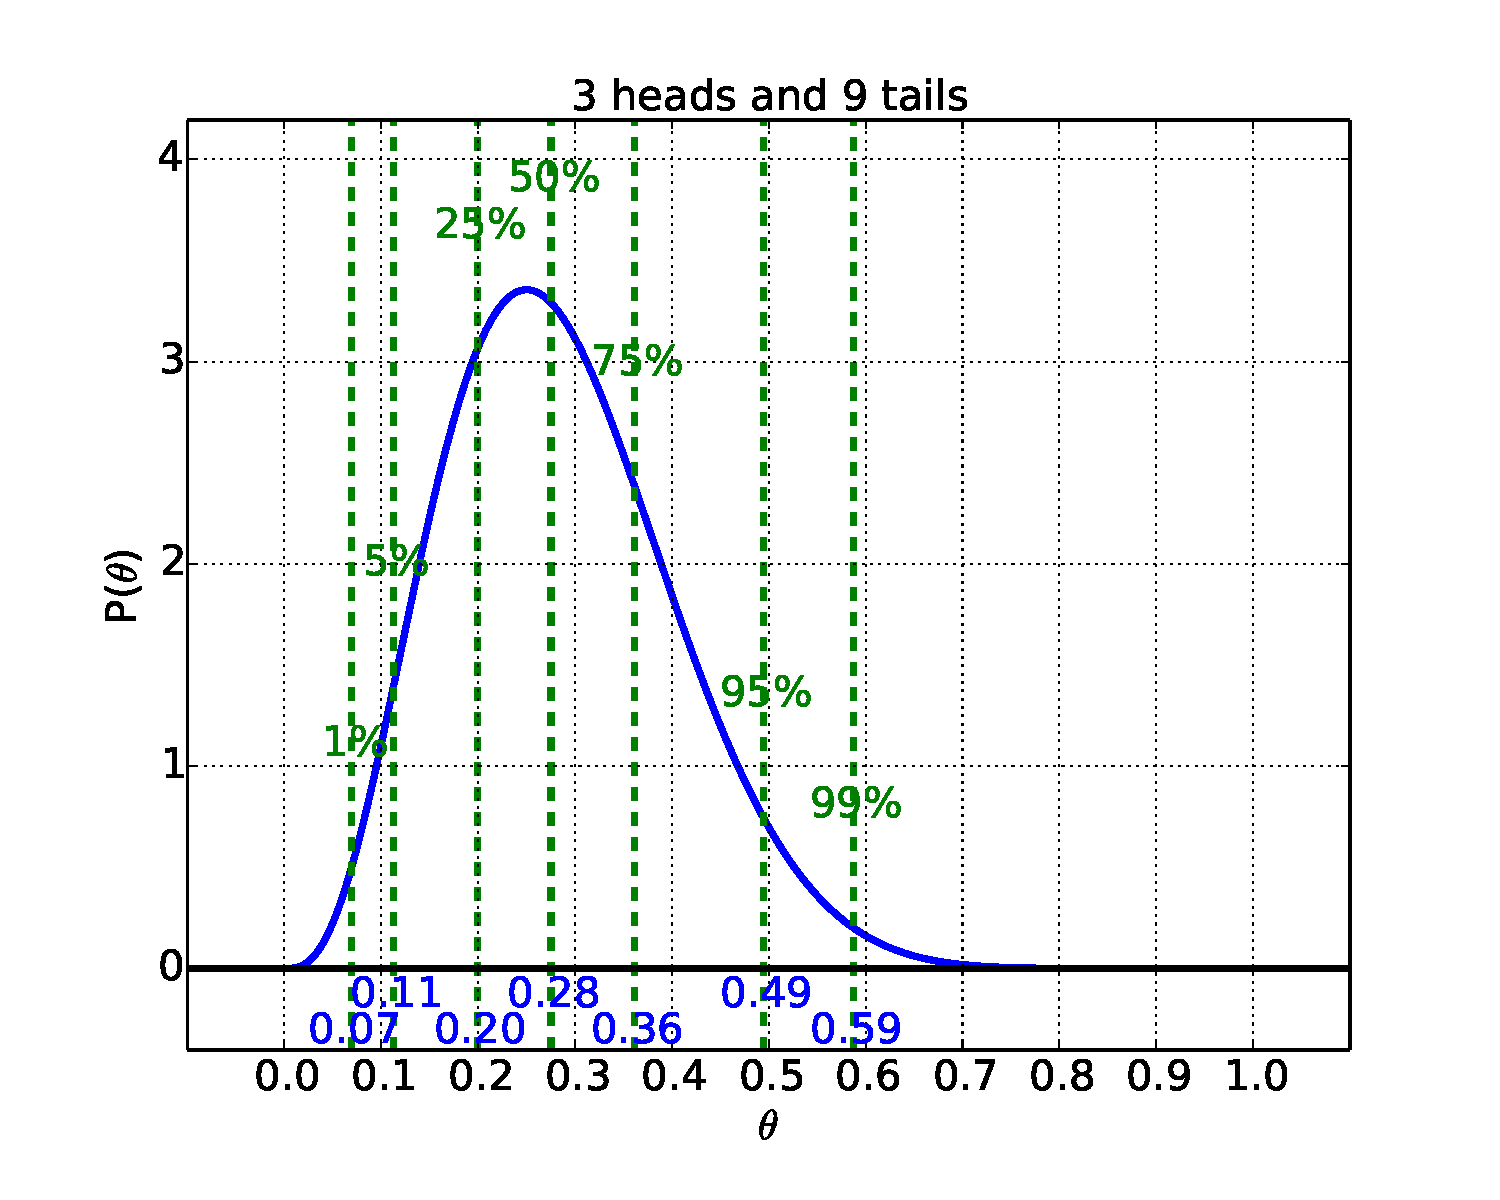
\includegraphics[height=3.66in]{beta_dist4}} & \begin{tabular}{cc}
\multicolumn{2}{c}{\textit{\textbf{Beta({\rm heads}=3,{\rm tails}=9)}}} \\
{\bf Value} & {\bf Area} \\ \hline
0.07 & 0.01 \\
0.11 & 0.05 \\
0.14 & 0.10 \\
0.20 & 0.25 \\
0.28 & 0.50 \\
0.36 & 0.75 \\
0.44 & 0.90 \\
0.49 & 0.95 \\
0.59 & 0.99 \\
\end{tabular}
\end{tabular}
\caption{Posterior probability distribution for the $\theta$ values of the bent coin - the probability that the coin will land heads.  The distribution is shown for data 3 heads and 9 tails.  The various quartiles are shown in the plot, and summarized in the accompanying table.}
\
\label{fig:coin_12_3_posterior_quartiles}
\end{figure*}

\newpage
\section{Best Estimates}\label{sec:bestest}

Perhaps surprisingly, there is not a single answer to the best estimate for $\theta$ given the posterier distribution, like the one shown in Figure~\ref{fig:coin_12_3_posterior_quartiles}.  There are several plausible measures, each with their own advantages.  Any specific estimate of a parameter (e.g. $\theta$) is denoted with a hat (e.g. $\hat{\theta}$) in the descriptions that follow.

\highlight{The Mode}{Also known as the \emph{maximum a-posteriori probability} (MAP) estimate, the \emph{mode} is the maximum of the posterior probability.   In the case of a Beta distribution with $h$ successes in $N$ trials, we have
\beqn
\hat{\theta}_{\rm mode} = \frac{h}{N}
\eeqn
}{Also known as the \emph{maximum a-posteriori probability} (MAP) estimate, the \emph{mode} is the maximum of the posterior probability.}

\highlight{The Mean}{Also known as the \emph{expected value} or \emph{average value}, the \emph{mean} of a distribution of a parameter $\theta$ is defined to be the sum of all of the possible values of $\theta$ times the posterior probability of $\theta$,
\beqn
\hat{\theta}_{\rm mean}= \sum_{\theta} \theta \times P(\theta|{\rm data})
\eeqn
It is one measure of the \emph{middle} of the distribution.  In the special case of a Beta distribution with $h$ successes in $N$ trials, we have
\beqn
\hat{\theta}_{\rm mean} = \frac{h+1}{N+2}
\eeqn
Intuitively this is the same as the MAP of the Beta distribution, with one more success and one more failure than actually observed.  Further, for the Beta distribution, the mean value $\hat{\theta}_{\rm mean}$ represents the predictive probability of a successful event on the \emph{next} observation.  
}{Also known as the \emph{expected value}, the \emph{mean} of a distribution of a parameter $\theta$ is defined to be the sum of all of the possible values of $\theta$ times the posterior probability of $\theta$, as in
\beqn
\hat{\theta}_{\rm mean}= \sum_{\theta} \theta \times P(\theta|{\rm data})
\eeqn
It is one measure of the \emph{middle} of the distribution. }

\highlight{The Median}{Also known as the 50\%-percentile, the median represents the middle of the distribution such that the probability of the parameter below the median equal to the probability of the parameter above the median.
\beqn
P(\theta\le\hat{\theta}_{\rm median}|{\rm data})=P(\theta\ge\hat{\theta}_{\rm median}|{\rm data})=0.5
\eeqn 
}{Also known as the 50\%-percentile, the median represents the middle of the distribution such that the probability of the parameter below the median equal to the probability of the parameter above the median.
\beqn
P(\theta\le\hat{\theta}_{\rm median}|{\rm data})&=&0.5\\
P(\theta\ge\hat{\theta}_{\rm median}|{\rm data})&=&0.5
\eeqn
}

\highlight{``Assume 2 successes and 2 failures'' median approximation}{
For the Beta distribution there is no simple form for the median, but a decent approximation which we will use is given by\cite{agresti2000simple}
\beqn
\hat{\theta}_{\rm median}&\approx&\frac{h+2}{N+4}
\eeqn
Intuitively this is the same as the MAP of the Beta distribution, with two more successes and two more failures than actually observed, and is thus referred to as the ``Assume 2 successes and 2 failures'' median approximation.
}{
For the Beta distribution there is no simple form for the median, but a decent approximation which we will use is given by
\beqn
\hat{\theta}_{\rm median}&\approx&\frac{h+2}{N+4}
\eeqn
Intuitively this is the same as the MAP of the Beta distribution, with two more successes and two more failures than actually observed, and is thus referred to as the ``Assume 2 successes and 2 failures'' median approximation.
}

Although each of these has their advantages, most notably ease of computation (especially for the mode and the mean), we will typically use the median of the distribution as the best estimate for the following reasons:
\be
\i the median is intuitive as literally the middle of the distribution
\i the median is not as sensitive to distributions that are highly asymmetric
\ee
In most practical examples it may not make much difference, and for some distributions (such as the Normal distribution described in Chapter~\ref{ch:priors_posteriors} (\emph{\nameref{ch:priors_posteriors}})) there is not difference - the mean \emph{is} the median which is also the mode.

\example{What is the best estimate of the probability of a bent coin flipping heads, given the observation of 9 tails and 3 heads?}

If we take the best estimate to be the median, then we have from the ``assuming 2 successes and 2 failures'' method,
\beqn
\hat{\theta}_{\rm median}&\approx&\frac{h+2}{N+4} \\
&=&\frac{5}{16} = 0.313
\eeqn
Notice that the maximum probability was at the somewhat lower value
\beqn
\hat{\theta}_{\rm mode} = \frac{h}{N}&=&\frac{3}{12}=0.25
\eeqn

One reason why the median is a better estimate in this case is because, as shown in Figure~\ref{fig:coin_12_3_posterior_quartiles}, there is more probability (i.e. area under the curve) to the right of the maximum than to the left, so the best estimate should be greater than the one given by the mode.

\section{Uncertainty in the Best Estimates}

To quantify the uncertainty in the best estimates, we need a value which represents the \emph{width} of the distribution.  Looking at Figure~\ref{fig:coin_30_10_posterior_quartiles} we'd like to provide a quick way of saying that the range of probable values lies somewhere between $\theta=0.2$ and $\theta=0.5$ - anything outside of this contributes only a small amount to the probability, or in other words, we are most confident that our best estimate of $\theta$ lies between those 0.2 and 0.5.  Depending on the application, the symmetry of the distribution, and other practical factors one may see a few potential measures of the \emph{width} of the distribution.

\highlight{Inter-Quantile Range}{The Inter-Quantile Range (ICR) is the range between the 25\% and 75\% quartiles, and represents 50\% of the probability.}{The Inter-Quantile Range (ICR) is the range between the 25\% and 75\% quartiles, and represents 50\% of the probability.}

In Figure~\ref{fig:coin_30_10_posterior_quartiles}, the Inter-Quantile Range  range is [0.29,0.40].  

\highlight{95\% Credible Interval (CI)}{The 95\% Credible Interval (CI) is the range between the 2.5\% and 97.5\% quantiles, and thus represents 95\% of the probability.  According to Table~\ref{table1} on page~\pageref{table1}, it is ``very likely'' that our best estimate lies in this range.}{The 95\% Credible Interval (CI) is the range between the 2.5\% and 97.5\% quantiles, and thus represents 95\% of the probability.  According to Table~\ref{table1} on page~\pageref{table1}, it is ``very likely'' that our best estimate lies in this range.}

In Figure~\ref{fig:coin_30_10_posterior_quartiles}, the 95\% Credible Interval is nearly [0.2,0.5].  

\highlight{Standard Deviation}{The standard deviation is a measure of the half-width of a distribution, most commonly used specifically with reference to the particular \emph{Normal} distribution.  This will be defined more precisely in Section~\ref{sec:normaldist} on page~\pageref{sec:normaldist}), and will thus not be defined in general here.}{The standard deviation is a measure of the half-width of a distribution, most commonly used specifically with reference to the particular \emph{Normal} distribution.  This will be defined more precisely in Section~\ref{sec:normaldist} on page~\pageref{sec:normaldist}), and will thus not be defined in general here.}

An approximate value for the standard deviation for the Beta distribution is 
\beqn
\sigma \approx \sqrt{\hat{\theta} (1-\hat{\theta})/N}
\eeqn
From Figure~\ref{fig:coin_30_10_posterior_quartiles}, and using the median as the best estimate, $\hat{\theta}$, we get
\beqn
\sigma \approx \sqrt{0.34 (1-0.34)/30} = 0.09
\eeqn

\highlight{Standard Deviation to Uncertainty}{
To convert this number to an uncertainty, it is a mathematical consequence that about 65\% of the area is within 1 value of $\sigma$, 95\% of the area is within 2 values of $\sigma$, and 99\% of the area within 3 values.}{
To convert this number to an uncertainty, it is a mathematical consequence that about 65\% of the area is within 1 value of $\sigma$, 95\% of the area is within 2 values of $\sigma$, and 99\% of the area within 3 values.}

So, of for the approximate 95\% CI for the case shown in Figure~\ref{fig:coin_30_10_posterior_quartiles} is
\beqn
[0.34 - 2\cdot 0.09, 0.34 + 2\cdot 0.09] = [0.16,0.52]
\eeqn
a bit more conservative range (larger uncertainty) than is given by the direct method of quantiles, but it much easier to calculate.

\section{Marginalization}

In Section~\ref{sec:marginalization_intro} we introduced the concept of marginalization, and in Section~\ref{sec:cancer_prob} we performed a discrete example of this.  In that section it was seen as simply a consequence of the sum and product rules.  It was a way of taking a probability that depended on several factors, and eliminating all but the single factor we're interested in.  If we have a {\em continuous} distribution, this process involves calculus and we will not cover it in detail, but it is the same process.  In the case of the distribution above, we have a distribution over a single variable, like ${\rm Beta}(\theta|h,t)$.  Imagine that we have a distribution that depends on {\em two} parameters, 
\beqn
{\rm MyDist}(\theta,\xi)
\eeqn
which specifies the probability of an event given each combination of the parameters, $\theta$ and $\xi$.  We'd have to do a three-dimensional plot to visualize this.  Many times, however, we want just the probability of one of the single parameters.  In those cases we will write
\beqn
P(\theta) &\sim& \left[{\rm MyDist}(\theta,\xi)\right]_{\mbox{\scriptsize marginalize over $\xi$}} 
\eeqn
where we are ``summing'' over all the values of the other parameters, leaving the details to the mathematicians, and simply using the result.  

Likewise we can {\em marginalize} the parameter $\theta$ to get the distribution of the other variable.  
\beqn
P(\xi) &\sim& \left[{\rm MyDist}(\theta,\xi)\right]_{\mbox{\scriptsize marginalize over $\theta$}} 
\eeqn



This becomes important in Chapter~\ref{ch:priors_posteriors} and Chapter~\ref{ch:parameter2}.


\section{Exercises}

\exercise{More Coin Flipping}{
Given the posterior shown in Figure~\ref{fig:coin_30_10_posterior_quartiles} for 10 heads and 20 tails, answer the following:
\be
\i The most likely estimate for the parameter $\theta$.  What does this mean?
\i Is it likely that this is a fair coin?
\i What is $P(0\le \theta \le 0.3)$ approximately?
\i What is $P(0.2\le \theta \le 0.35)$ approximately?
\i What is the {\em median} value?  What are the quartiles?
\ee
}


\begin{figure*}
\begin{tabular}{cp{1in}}
\raisebox{-2in}{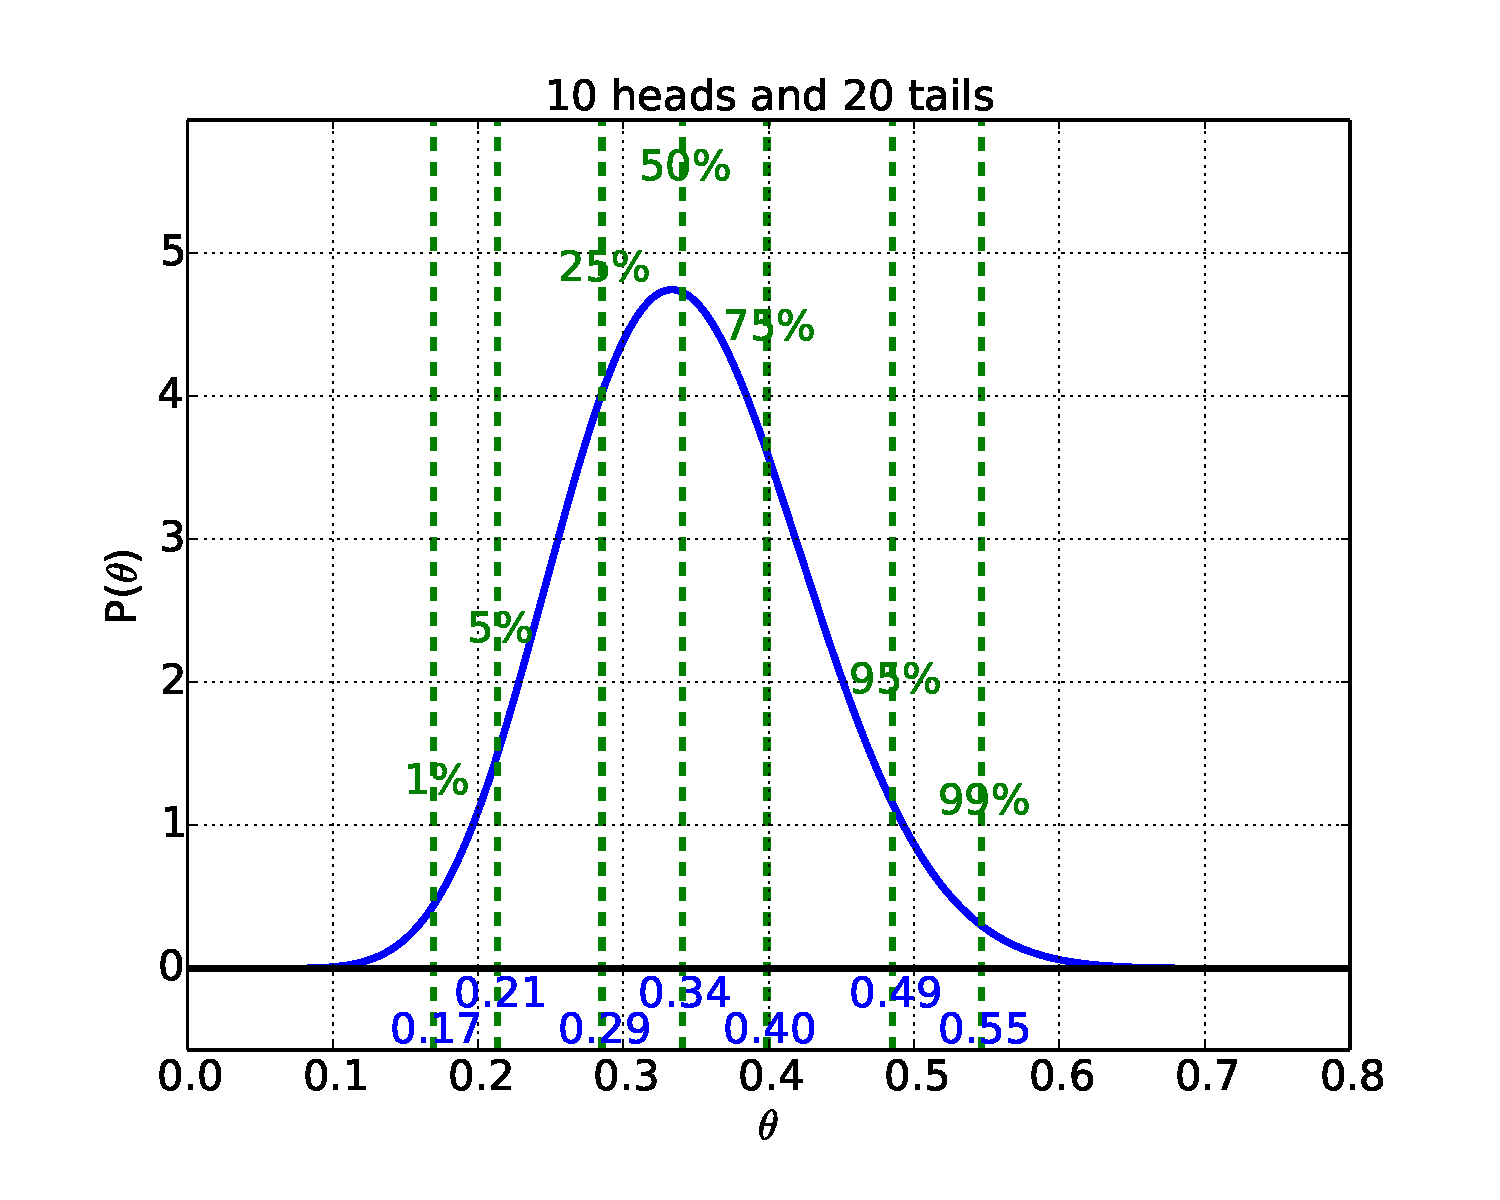
\includegraphics[height=3.66in]{beta_dist5}} & 
\begin{tabular}{cc}
\multicolumn{2}{c}{\textit{\textbf{Beta({\rm heads}=10,{\rm tails}=20)}}} \\
{\bf Value} & {\bf Area} \\
0.17 & 0.01 \\
0.21 & 0.05 \\
0.24 & 0.10 \\
0.29 & 0.25 \\
0.34 & 0.50 \\
0.40 & 0.75 \\
0.45 & 0.90 \\
0.49 & 0.95 \\
0.55 & 0.99 \\
\end{tabular}
\end{tabular}
\caption{Posterior probability distribution for the $\theta$ values of the bent coin - the probability that the coin will land heads.  The distribution is shown for data 10 heads and 20 tails.  The various quartiles are shown in the plot, and summarized in the accompanying table.}
\
\label{fig:coin_30_10_posterior_quartiles}
\end{figure*}

\section{Computer Examples}
\begin{fullwidth}
\begin{lstlisting}
from sie import *
\end{lstlisting}

\subsection{Beta Distribution Example}


\subsubsection{3 heads and 9 tails}


Plot a beta distribution with 3 heads and 9 tails...

\begin{lstlisting}
dist=beta(h=1,N=3)
distplot(dist,xlim=[0,1],show_quartiles=False)
\end{lstlisting}

\begin{center}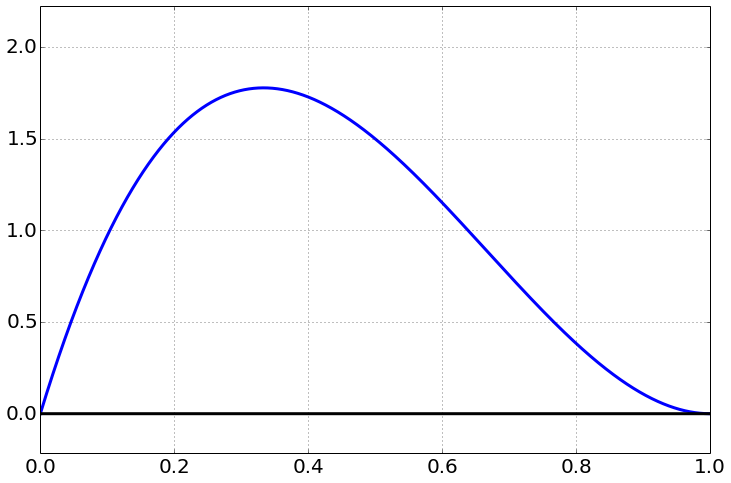
\includegraphics[width=4.5in]{Introduction_to_Parameter_Estimation/Introduction_to_Parameter_Estimation_fig0.png}\end{center}

The median of this distribution...

\begin{lstlisting}
dist.median()
\end{lstlisting}

\begin{verbatim}
0.27527583248615201
\end{verbatim}

the 95% credible interval, with the median in the middle,

\begin{lstlisting}
credible_interval(dist)
\end{lstlisting}

\begin{verbatim}
(0.067585986488542985, 0.38572756813238962, 0.80587955031675662)
\end{verbatim}

\subsubsection{1 heads and 3 tails}


This should be about the same fraction as the previous example, but broader

\begin{lstlisting}
dist=beta(h=1,N=4)
distplot(dist,xlim=[0,1])
\end{lstlisting}

\begin{verbatim}
<matplotlib.figure.Figure at 0x108768cd0>\end{verbatim}

\begin{center}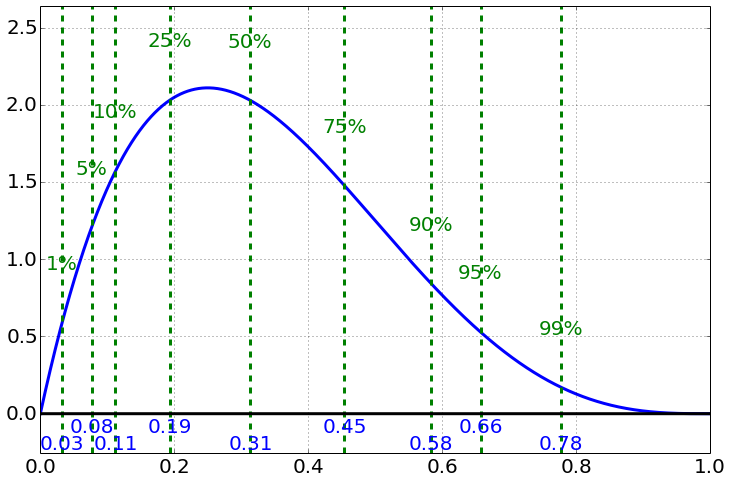
\includegraphics[width=4.5in]{Introduction_to_Parameter_Estimation/Introduction_to_Parameter_Estimation_fig1.png}\end{center}

\begin{lstlisting}
credible_interval(dist)
\end{lstlisting}

\begin{verbatim}
(0.052744950526316919, 0.31381017045569742, 0.71641793611808946)
\end{verbatim}

\begin{lstlisting}

\end{lstlisting}


\end{fullwidth}
